\chapter{Implementation}

In this chapter, we first give a high level overview of the possibilities for parallelization and data reuse in the implementation of definition-based cross-correlation algorithm, introduced in section \ref{sec:cross_corr_def}. We then describe a basic implementation of the definition-based algorithm with all its problems. Next, we try to mitigate the problems of the basic implementation by introducing a simple implementation based on Warp Shuffle instructions. We continue with several optimizations of this implementation. Lastly we implement a solution to the problem of low occupancy for small inputs and go through some additional possibilities for optimization of this solution.


The definition-based algorithm has several properties which allow for parallelization, optimization through data reuse and distribution of work. Figure \ref{fig:cross_corr_shifts} depicts the output matrix with corresponding relative shift of the two input matrices, which defines the computed overlap. As described in Section \ref{sec:cross_corr_opt}, each element of the output matrix can be computed independently in parallel.

\begin{figure}[ht]
	\fontsize{6}{8}\selectfont
	\centering
	\def\svgwidth{0.55\textwidth}
	% Must be relative to current directory
	% as input ignores graphicspath, which is
	% only for includegraphics{}
	\input{./img/overlap-Shifts.pdf_tex}
	\caption{Result matrix with corresponding relative shifts.}
	\label{fig:cross_corr_shifts}
\end{figure}

Each overlap defines a unique set of element pairs which are to be multiplied. Each of these pairs of overlapping elements belongs to exactly one overlap of the two matrices.


\section{Parallelization}
\label{sec:implementation_parallelism}
In this section, we first highlight the independent parallel tasks present in the definition-based cross-correlation algorithm.  

\subsection{Two matrices}
When we focus on the computation of cross-correlation between two matrices, called \textit{one-to-one} in the rest of the thesis, we can reformulate the definition-based algorithm as a problem with two levels of independent parallel tasks, as shown in Figure \ref{fig:cross_corr_one_to_one_tasks}. The top level represents the single output matrix, which with only two input matrices represents the result of the whole computation. The second level of tasks, represented by orange boxes, contains one box for each relative shift of the two input matrices, or in other words each orange box corresponding to a single element of the output matrix. Each shift defines an overlap of the two input matrices, which in turn defines a set of independent subtasks, each subtask representing an overlapping pair of elements of the two input matrices. In Figure \ref{fig:cross_corr_one_to_one_tasks}, the subtasks representing pairs of overlapping elements are represented by yellow boxes. Every such subtask belongs to exactly one second level task, creating a tree structure. The set of subtasks which are children of the same orange box defines a submatrix in both input matrices, as shown in Figure \ref{fig:cross_corr_shifts}.


When we look at the operations, every yellow box represents a single multiplication and every orange box represents a sum of the results of all of its children. 

\begin{figure}[ht]
	\fontsize{5}{6}\selectfont
	\centering
	\def\svgwidth{0.6\textwidth}
	% Must be relative to current directory
	% as input ignores graphicspath, which is
	% only for includegraphics{}
	\input{./img/overlap-Tasks.pdf_tex}
	\caption{Tasks hierarchy in definition-based one-to-one cross-correlation.}
	\label{fig:cross_corr_one_to_one_tasks}
\end{figure}

The goal is to distribute the tasks between workers in such a way that we maximize parallelism, maximize data reuse and minimize the need for communication and synchronization between workers.

\subsection{Many matrices}

With more than two matrices, we add additional tasks to the top level of the task hierarchy shown in Figure \ref{fig:cross_corr_one_to_one_tasks}, creating a forest of trees. As described in Section \ref{sec:cross_corr_forms}, there are several forms of cross-correlation between multiple matrices. For us, the most important of these are:
\begin{enumerate}
	\item \textit{one-to-many} (Figure \ref{fig:implementation_one_to_many}),
	\item \textit{n-to-mn} (Figure \ref{fig:implementation_n_to_mn}),
	\item \textit{n-to-m} (Figure \ref{fig:implementation_n_to_m}).
\end{enumerate}

\begin{figure}
	\centering	
	\begin{subfigure}{0.4\textwidth}
		\centering
		\def\svgwidth{0.5\textwidth}
		% Must be relative to current directory
		% as input ignores graphicspath, which is
		% only for includegraphics{}
		\input{./img/overlap-OneToOne.pdf_tex}
		\caption{One to one.}
		\label{fig:implementation_one_to_one}
	\end{subfigure}
	\hfill
	\begin{subfigure}{0.4\textwidth}
		\centering
		\def\svgwidth{0.5\textwidth}
		% Must be relative to current directory
		% as input ignores graphicspath, which is
		% only for includegraphics{}
		\input{./img/overlap-OneToMany.pdf_tex}
		\caption{One to many.}
		\label{fig:implementation_one_to_many}
	\end{subfigure}
	\hfill
	\begin{subfigure}{0.4\textwidth}
		\centering
		\def\svgwidth{0.7\textwidth}
		% Must be relative to current directory
		% as input ignores graphicspath, which is
		% only for includegraphics{}
		\input{./img/overlap-NtoMN.pdf_tex}
		\caption{N to MN.}
		\label{fig:implementation_n_to_mn}
	\end{subfigure}
	\hfill
	\begin{subfigure}{0.4\textwidth}
		\centering
		\def\svgwidth{0.7\textwidth}
		% Must be relative to current directory
		% as input ignores graphicspath, which is
		% only for includegraphics{}
		\input{./img/overlap-NToM.pdf_tex}
		\caption{N to M.}
		\label{fig:implementation_n_to_m}
	\end{subfigure}
	
	\caption{Forms of cross-correlation.}
	\label{fig:implementation_forms}
\end{figure}

The \textit{one-to-many} type together with the \textit{one-to-one} type, shown in Figures \ref{fig:implementation_one_to_many} and \ref{fig:implementation_one_to_one} respectively, are subtypes of the \textit{n-to-mn} type and \textit{n-to-m}, as implementations of both of these general types can be used to compute the two simpler types. We separate the \textit{one-to-one} and \textit{one-to-many} types as they offer a greater possibility for caching the single left input matrix.

All of the described types can be partitioned into many \textit{one-to-one} cross-correlations, as shown in Figure \ref{fig:cross_corr_many_tasks}. For both \textit{n-to-mn} and \textit{n-to-m} types, the number of green top level tasks, corresponding to the number of result matrices, is equal to $n*m$. To reiterate, the difference between the \textit{n-to-mn} and \textit{n-to-m} types is that in the \textit{n-to-mn} type, each of the \textit{n} left input matrices is cross-correlated with a different set of \textit{m} right input matrices, whereas in the \textit{n-to-m} type, all \textit{n} left input matrices are cross-correlated with the same \textit{m} right input matrices. Based on this, the \textit{n-to-m} type allows for greater data reuse, as each right input matrix is used multiple times compared to being used just once in the \textit{n-to-mn} type. 

\begin{figure}[ht]
	\centering
	\def\svgwidth{0.8\textwidth}
	% Must be relative to current directory
	% as input ignores graphicspath, which is
	% only for includegraphics{}
	\input{./img/overlap-ManyTasks.pdf_tex}
	\caption{Task hierarchy of types with many matrices.}
	\label{fig:cross_corr_many_tasks}
\end{figure}

As in the case of \textit{one-to-one} type, the meaning of the boxes is as follows:

\begin{itemize}
	\item Each green box represents a pair of input matrices, or equivalently a single output matrix;
	\item Each orange box represents an element in the output matrix, or equivalently a relative shift of the two input matrices;
	\item Each yellow box represents a pair of overlapping elements from the two input matrices.
\end{itemize}

All boxes on a given level can be processed completely independently.  Results of the orange boxes have to be written into the output matrix represented by their green box parent. Each orange box represents a different element of the parent matrix, which allows the writes corresponding to different orange box tasks to be executed without any collisions. All results of the yellow box children of an orange box have to be summed together.

% Segway to data reuse and workers

As the number of tasks cannot be reduced, the only directions for optimization are parallelization and data reuse. Even through tasks can be processed independently and in parallel, many tasks can share and reuse data from other tasks. For example, orange boxes from different subtrees representing the same shift between input matrices and sharing the same left input matrix can be computed by reusing the data from the left matrix. Relationships such as this can be used to group tasks into \textbf{jobs} for workers to reuse data or pass data to other neighboring workers to reduce the required memory throughput and keep data closer to the execution units. 

\section{Data reuse}
\label{sec:data_reuse}
To fully utilize the GPU hardware, we cannot rely on parallelization alone, but must keep the data as close as possible to the execution units for fast access. To achieve this goal, we have to group tasks defined in the previous section \ref{sec:implementation_parallelism} into cooperating groups, mostly for sharing input data. We call these groups \textbf{jobs}.

The two basic levels on which tasks are grouped into jobs in our implementations are:
\begin{itemize}
	\item overlap,
	\item row group or column group.
\end{itemize}

The following subsections describe groupings based on each of these units.

\subsection{Overlap}
\label{sec:data_reuse_overlap}

With the basic job size of single \textit{overlap}, each job contains a single element in the output matrix. This corresponds to a single orange box in the task hierarchy in Figure \ref{fig:cross_corr_many_tasks}. The job then represents all tasks in the subtree with the assigned orange box as its root.

With \textit{multimat overlap} job size, multiple overlaps (orange boxes) from different output matrices (green boxes) are grouped into a single job. To enable data reuse, overlaps representing the same shift between different matrices are grouped, as shown in Figure \ref{fig:job_size_modifiers}. There are two versions of this optimization:
\begin{itemize}
	\item multimat-right, designed for \textit{n-to-mn} computation type, where job contains overlaps with the same shift between single left input matrix and multiple right input matrices, shown in Figure \ref{fig:job_size_modifiers_n_to_mn};
	\item multimat-both, designed for \textit{n-to-m} computation type, where job contains overlaps with the same shift between multiple left input matrices and multiple right matrices, shown in Figure \ref{fig:job_size_modifiers_n_to_m}.
\end{itemize}

Another way to reuse data is to compute multiple overlaps which are close to each other in a single output matrix. Their proximity in the output matrix corresponds to the shifts of the input matrices being very similar, which in turn means that most of the input data is shared between the overlaps, as shown in Figure \ref{fig:multirow_shared_input}. This grouping is also shown in Figure \ref{fig:job_size_modifiers}. Our implementation groups overlaps from multiple consecutive rows of a single column of the output matrix into a single job. The reasons for this grouping choice are further expanded in Section \ref{sec:multirow_right}.
% TODO: Maybe multirow-right and multirow-both



The \textit{multimat} and \textit{multirow} optimizations can be combined as shown in Figure \ref{fig:job_size_modifiers}.



\begin{figure}
	\centering	
	\begin{subfigure}{0.4\textwidth}
		\centering
		\def\svgwidth{\textwidth}
		\fontsize{8}{10}\selectfont
		% Must be relative to current directory
		% as input ignores graphicspath, which is
		% only for includegraphics{}
		\input{./img/overlap-JobSizeOverlapSimple.pdf_tex}
		\caption{Grouping in \textit{n-to-mn} type.}
		\label{fig:job_size_modifiers_n_to_mn}
	\end{subfigure}
	\hfill
	\begin{subfigure}{0.4\textwidth}
		\centering
		\def\svgwidth{\textwidth}
		\fontsize{8}{10}\selectfont
		% Must be relative to current directory
		% as input ignores graphicspath, which is
		% only for includegraphics{}
		\input{./img/overlap-JobSizeBoth.pdf_tex}
		\caption{Grouping in \textit{n-to-m} type.}
		\label{fig:job_size_modifiers_n_to_m}
	\end{subfigure}
	
	\caption{Grouping of overlaps into jobs.}
	\label{fig:job_size_modifiers}
\end{figure}

\begin{figure}[ht]
	\centering
	\def\svgwidth{0.4\textwidth}
	\fontsize{8}{10}\selectfont
	% Must be relative to current directory
	% as input ignores graphicspath, which is
	% only for includegraphics{}
	\input{./img/overlap-DataSharedByOverlaps.pdf_tex}
	\caption{Input data shared between neighboring overlaps.}
	\label{fig:multirow_shared_input}
\end{figure}

\subsection{Row group and Column group}
\label{sec:data_reuse_row_column_group}

% With work distribution, jobs created from the same overlap do not share any input data, but share data with the jobs with the same ID from neighboring overlaps

With overlaps as the tasks grouped into jobs, load balancing becomes a problem. The amount of work required by each job may differ massively, as illustrated by the two tasks shown by the two overlaps in Figure \ref{fig:row_subset_tasks}. This leads to problems with occupancy once jobs with small amount of work are finished. 

We implement an alternative where instead of grouping overlaps into jobs, we go one step lower in the task hierarchy and group the individual tasks representing multiplication of one overlapping pair of input elements (yellow box) into jobs. This change results in the computation of a single overlap being split into several smaller jobs, improving load balancing between jobs while also increasing parallelism. One problem of this change is the required final reduce operation to consolidate the results of all jobs computing parts of the same overlap.

To enable additional optimizations described in the following sections of this chapter, we choose to group the yellow box tasks into jobs by whole rows of the overlap, with the maximum number of rows making up a job configurable through algorithm argument. This grouping is illustrated in Figure \ref{fig:row_subset_tasks}, where \textit{Max job rows} is the argument of the algorithm. Each overlap with $r$ overlapping rows of the two input matrices is split into $\lceil \frac{r}{max\_job\_rows} \rceil$ jobs, with each job containing at most \textit{max\_job\_rows} consecutive rows. With this distribution, each job represents a submatrix of the overlap with the same number of columns as the original overlap. This also means that all overlaps with the same number of rows will be split into the same number of jobs.

For data reuse, one important observation is that jobs from the same overlap do not share any input data, but jobs with the same ID from neighboring overlaps in the same row of the output matrix, i.e. with the same number of rows in the overlap, will share most of the input data, as shown in Figure \ref{fig:row_subset_data_reuse}.

\begin{figure}[ht]
	\centering
	\def\svgwidth{0.7\textwidth}
	% Must be relative to current directory
	% as input ignores graphicspath, which is
	% only for includegraphics{}
	\input{./img/overlap-JobSizeRowSubset.pdf_tex}
	\caption{Grouping of rows of tasks into jobs.}
	\label{fig:row_subset_tasks}
\end{figure}

\begin{figure}[ht]
	\centering
	\def\svgwidth{0.4\textwidth}
	\fontsize{8}{10}\selectfont
	% Must be relative to current directory
	% as input ignores graphicspath, which is
	% only for includegraphics{}
	\input{./img/overlap-DataSharedRowSubsets.pdf_tex}
	\caption{Data shared between jobs with the same ID from neighboring overlaps.}
	\label{fig:row_subset_data_reuse}
\end{figure}

For some optimizations, it is better to group tasks by columns instead of rows. From the data reuse point of view, it is symmetrical to the grouping by rows. Again, column groups from the same shift do not share any input data, but column groups with the same ID from two neighboring overlaps in the same column of the output matrix share most of their input data.

The \textit{multimat} optimization introduced in Section \ref{sec:data_reuse_overlap} can also be used with both row group and column group task grouping. The \textit{multimrow} optimization is unfortunately incompatible with both row group and column group task grouping.

\subsection{Workers}

Jobs defined in the previous section are assigned to one level of the CUDA thread group hierarchy, described in Section \ref{sec:thread_hierarchy}. The CUDA thread hierarchy contains the following groups of threads:
\begin{enumerate}
	\item thread,
	\item warp,
	\item thread block,
	\item grid.
\end{enumerate}

We call each member from the chosen thread hierarchy level, i.e. the thread, warp, thread block, or grid, a \textbf{worker}. Each worker is assigned at most one job, but due to the fixed warp size and limited size of thread blocks, we might need to start more workers than jobs and later stop the redundant workers. Based on the choice of worker size, we can utilize smaller groups in the hierarchy to compute tasks of the assigned job, and primitives provided by larger groups to exchange input data or combine results with other workers.

\subsection{List of implementations}
\label{sec:algorithm_list}

The different implementations of the definition-based cross-correlation utilize different job sizes, worker types and different ways of assigning jobs to workers. The chosen parameters then lead to different ways of cooperation, communication, synchronization, work distribution and load balancing. Following is the list of algorithms implemented in this thesis with their choice of job size and worker type. Each algorithm is described in more detail in the following sections of this chapter.

\begin{center}
	\begin{tabular}{|p{3cm}|c|c|} 
		\hline
		Algorithm&Job size&Worker type\\ [0.5ex] 
		\hline\hline
		Basic &overlap&thread \\ 
		\hline
		\multirow{6}*{Warp shuffle}&overlap&\multirow{6}*{thread}\\
		&multimat overlap&\\
		&multirow overlap&\\
		&multimat multirow overlap&\\
		&row group&\\
		&multimat row group&\\
		\hline
		\multirow{2}*{Warp per shift}&overlap&\multirow{2}*{warp}\\
		&row group&\\
		\hline
		\multirow{3}{3cm}{Warp per shift with shared memory}&overlap&\multirow{3}*{warp}\\
		&column group&\\
		&multimat column group&\\
		\hline
		Block per shift&overlap&thread block\\
		\hline
	\end{tabular}
\end{center}

Algorithms with multiple job sizes are provided in multiple implementations, each implementing different optimization for data reuse.

% TODO: Maybe expand what the choice for each algorithm means

\section{Basic algorithm}
\label{sec:basic_alg}

A basic implementation of definition based cross-correlation of two input matrices, in our naming scheme corresponding to the \textit{one-to-one} type, utilizes two dimensional grid of two dimensional thread blocks to start one thread for each element of the output matrix. The overlap to be computed by given thread is derived from the position of the output matrix element, as shown in Figure \ref{fig:basic_algorithm_overlaps}. The thread then iterates over the overlapping parts of the two input matrices, multiplying the overlapped elements and accumulating the result which is then written to the assigned output matrix element.

\begin{figure}[ht]
	\fontsize{6}{8}\selectfont
	\centering
	\def\svgwidth{0.55\textwidth}
	% Must be relative to current directory
	% as input ignores graphicspath, which is
	% only for includegraphics{}
	\input{./img/overlap-Shifts.pdf_tex}
	\caption{Examples of overlaps corresponding to output matrix elements.}
	\label{fig:basic_algorithm_overlaps}
\end{figure}

This implementation allows for great amount of parallelism, as each element of the output matrix is computed independently.
The disadvantages on the other hand are no data reuse, thread divergence, and a large difference between workloads assigned to each thread.


The problem with no data reuse is illustrate by Figure \ref{fig:warp_shuffle_shuffle}. The figure shows elements of the left input matrix (in blue) and right input matrix (in red) accessed by thread 0 and thread 1 in iterations 0 to 11. As memory accesses are done in units of 32 threads, also known as warp, when we extrapolate this example, the 32 values loaded from the left input matrix in global memory will contain 31 values read in the previous iteration by the threads of this warp. In other words, we are moving a window of 32 elements across each row of the left matrix 1 element per iteration and reading the window from global memory in each iteration. This problem is exacerbated with thread blocks with the \textit{x} component of their size not multiple of warp size. In this situation, threads of a warp are assigned overlaps which differ in number of rows, and consequently in the rows of the input matrices which are to be read in the given iteration. This means that threads of a single warp access two or more different rows of the left input matrix in each iteration, leading to non-coalesced loads.

In the right input matrix, all threads of the warp will read the same value from global memory in each iteration, resulting in 32 reads of the same block of global memory when reading 32bit values. 

The exact pattern of reads from global memory differs based on the overlaps processed by the threads of the warp, but will always result in repeated reads of the same block of global memory.


The problem of thread divergence is also illustrated by Figure \ref{fig:warp_shuffle_shuffle} with iterations 3, 7 and 11.
The basic implementation of looping over a two dimensional matrix with two nested for loops results in thread 0 reading an element from each input matrix, computing multiplication and accumulating the result in these iterations, while thread 1 has no data to process on this row and its inner for loop being masked due to the range condition being false. While we show only two threads in Figure \ref{fig:warp_shuffle_shuffle}, the situation is much worse as 31 threads of the 32 threads of the warp will be masked and not doing anything in the last iteration. All threads of the warp will go through both for loops based on the size of the largest overlap in the given axis processed by any thread of the warp. 

Last significant problem of the Basic algorithm, largely connected with the previous problem, is that overlaps differ in size. From overlaps containing one element from each input matrix to overlap of the whole input matrices, this difference in workload size means that some threads will finish rather quickly, while small number of threads computing the largest overlaps will take much longer. For example warps of threads assigned overlaps in the first or last row of the output matrix will only read a single row of each input matrix, and finish quickly, while warps assigned overlaps in the middle of the output matrix will read most elements of each input matrix and run for much longer. This results in problems with occupancy of the GPU.
  
  
Slight modification of this algorithm to allow for an \textit{n-to-mn} computation is implemented by the original thesis \citet{misko}.



\begin{figure}[ht]
	\centering
	\def\svgwidth{0.5\textwidth}
	\fontsize{8}{10}\selectfont
	% Must be relative to current directory
	% as input ignores graphicspath, which is
	% only for includegraphics{}
	\input{./img/overlap-WarpShuffleShuffle.pdf_tex}
	\caption{The iteration in which each input matrix element is accessed by two neighboring threads.}
	\label{fig:warp_shuffle_shuffle}
\end{figure}



\section{Warp shuffle algorithm}
\label{sec:warp_shuffle_alg}

This section describes the implementation of definition-based cross-correlation utilizing Warp Shuffle instructions, which tries to fix the problems of the Basic algorithms described in the previous section. We first introduce a simple version of the implementation, later improving it step by step with optimizations evaluated in Section \ref{sec:results_warp_shuffle}.

In the simplified implementation, Warp Shuffle instructions are utilized to shuffle data loaded from the left matrix and broadcast data loaded from the right matrix between threads in a warp. As shown in Section \ref{sec:algorithm_list}, each CUDA thread is assigned an overlap to compute the same way as in the Basic algorithm.

The main idea behind this algorithm can be illustrated by using Figure \ref{fig:warp_shuffle_shuffle}. The two threads computing overlaps with shifts $[0,1]$ and $[1,1]$ process elements of the two input matrices in the indicated iterations of a \textit{for loop} in the code.


The element from the left matrix read by the thread processing shift $[x, y]$ in iteration \textit{i} is required by thread processing shift $[x + 1,y]$ in iteration \textit{i + 1}. This holds for any two neighboring shifts and maps exactly onto the Warp Shuffle Down function, described in Section \ref{sec:thread_cooperation}. When looking at the right matrix in any given iteration, both shifts require the exact same element from the right matrix. This broadcast can be implemented using the general Warp Shuffle function with direct source lane indexing. Iterations 3, 7, and 11 are skipped by thread 1 to preserve this property.

% Distribution of shifts between threads and blocks, block dimensions etc.

To utilize these properties, threads of a single warp process 32 consecutive overlaps in a row of the output matrix, as shown in Figure \ref{fig:warp_shuffle_simple_dist}. The \textit{x} axis of \textit{thread block size} is set to \textit{warp size} for simplified grouping of threads into warps. The number of warps per thread block is configurable using a run-time algorithm argument. The grid size is set so that the output matrix is fully covered by threads. Any redundant threads do not write to the output matrix and during computations are handled by the bound checked reads described next.

% TODO: Maybe show how this solves the problem of first iterations
The problem of iteration 3, 7 and 11 in Figure \ref{fig:warp_shuffle_shuffle}, in which thread 1 does not have any value to compute, can be solved in several ways. If we were programming for a CPU, we would give the two for loops implementing the two worker threads different bounds so that the second worker stops earlier. A more GPU friendly implementation needs to prevent thread divergence. This is achieved by executing the range check only once when loading the data from the left matrix into a register of the thread. If the thread is loading value outside the matrix, it loads 0 instead. This makes the result of the multiplication performed in each step 0 which is then added to the sum, effectively skipping the iteration while preventing thread divergence. This also handles any extra threads introduced due to the fixed size of thread block and overlap sizes not divisible by warp size.

\begin{figure}[ht]
	\centering
	\def\svgwidth{0.8\textwidth}
	% Must be relative to current directory
	% as input ignores graphicspath, which is
	% only for includegraphics{}
	\input{./img/overlap-WarpShuffleWarps.pdf_tex}
	\caption{Distribution of overlaps in a 7 by 59 output matrix between threads of thread blocks and warps.}
	\label{fig:warp_shuffle_simple_dist}
\end{figure}

\subsection{Algorithm steps}
\label{sec:simplified_warp_shuffle_steps}

The following description assumes \textit{warp size} to be 32, as is the case for all currently existing Nvidia GPUs. To utilize coalesced loading from global memory, the buffer that is shuffled between threads of a warp, containing data from the left input matrix, is split into two parts of 32 items each, which together function as a single 64 item ring buffer. We call the parts \textit{top} and \textit{bottom}, where new data is always loaded to the top part and then shuffled towards the bottom part, as shown in Figure \ref{fig:shuffle_buffer}. As described above, any out of bounds loads are range checked and load value 0 instead using the following code:
\begin{lstlisting}[
style=cuda
]

template<typename T>
__device__ T load_with_bounds_check(const T* source, int idx, size_t size) {
	return (idx >= 0 && idx < size) ? source[idx] : 0;
}
\end{lstlisting}


When loading a buffer, bound checked load shown above is used to load 32 consecutive values (or load the value 0 if out of bounds), storing one item per thread into a register. This is implemented by the following code:
\begin{lstlisting}[
style=cuda
]
T thread_left_bottom = load_with_bounds_check(
	left_row,
	warp_x_left + warp.thread_rank(),
	matrix_size.x
);

\end{lstlisting}

Each thread holds single value of \texttt{thread\_left\_bottom}. Same is done for \texttt{thread\_left\_top}, creating a 64 item ring buffer distributed between threads of a warp which is shuffled using the Warp Shuffle instructions as shown in Figure \ref{fig:shuffle_buffer}.

\begin{figure}[ht]
	\centering
	\def\svgwidth{\textwidth}
	% Must be relative to current directory
	% as input ignores graphicspath, which is
	% only for includegraphics{}
	\input{./img/overlap-ShuffleBuffer.pdf_tex}
	\caption{Shuffling of the left buffer.}
	\label{fig:shuffle_buffer}
\end{figure}

For the data loaded from the right matrix, which we use for broadcasting, we require only a single value per thread, as in the 32 iterations of the innermost loop, we will broadcast only these 32 values, whereas we need 64 from the left matrix as the 32 values loaded into the top part will be shifted all the way to the bottom part.

The outer loops of the algorithm are illustrated by the following code:

\begin{lstlisting}[
style=cuda
]
// Compute bounds of the overlaps processed by warp
// Comput thread output position

T sum = 0;
/* for each overlapping row in the right input matrix */
for (size_t warp_y_right ... ) {

	// Corresponding row in the left input matrix
	int warp_y_left = warp_y_right + warp_min_shift.y;
	
	// First column in the left input matrix 
	// corresponding to the first column in the right input matrix
	int warp_x_left = warp_x_right_start + warp_min_shift.x;
	
	// Preload 1 value to each thread from the input left matrix
	T thread_left_bottom = load_with_bounds_check(left_matrix, ...);
	
	for (size_t warp_x_right ...; warp_x_right += warp.size()) {
		int warp_x_left = warp_x_right + warp_min_shift.x;
		
		T thread_left_top = load_with_bounds_check(left_matrix, ...);
		T thread_right = load_with_bounds_check(right_matrix, ...);
		
		/* Main loop shown below, with warp.size() iterations */
	}
}

if (/* thread output not out of bounds */) {
	out_matrix[output_offset] = sum;
}
\end{lstlisting}

The 32 threads of a warp are assigned 32 consecutive overlaps, where thread i computes overlap with shift $[warp\_min\_shift.x + i, warp\_min\_shift.y]$. Thread 31 (or possibly earlier thread if there are redundant threads in the warp) is then assigned shift $[warp\_max\_shift.x, warp\_max\_shift.y]$, which in a warp without redundant threads is equal to $[warp\_min\_shift.x + 31, warp\_max\_shift.y]$, otherwise the \textit{x} component is clamped to the maximum shift defined by the output matrix. The \textit{min} and \textit{max} shifts are then used to compute a submatrix of the right input matrix which contains elements required by any thread in the warp, shown in Figure \ref{fig:common_submatrix}. We call this the \textit{warp submatrix}.

\begin{figure}[ht]
	\centering
	\def\svgwidth{0.5\textwidth}
	% Must be relative to current directory
	% as input ignores graphicspath, which is
	% only for includegraphics{}
	\input{./img/overlap-WarpShuffleCommonSubmatrix.pdf_tex}
	\caption{Submatrix of input data used by any thread in the warp.}
	\label{fig:common_submatrix}
\end{figure}

The two loops in the code above then iterate over this submatrix of the right input matrix, outer loop iterating over rows of the submatrix and the inner loop iterating in buffer load size steps over the columns of the submatrix. As described above, both buffers are loaded 32 items at the time to allow for coalesced loads.


The innermost loop, which we call the \textit{main loop} in the code above, then does 32 (warp size) iterations illustrated by the following code:

\begin{lstlisting}[
style=cuda
]
for (size_t i = 0; i < warp.size(); ++i) {
	// Broadcast right buffer
	auto right_val = warp.shfl(thread_right, i);
	sum += thread_left_bottom * right_val;

	// Shift left buffer
	// General shuffle does module on source lane argument
	// Thread 0 needs to connect the top buffer to the bottom buffer
	thread_left_bottom = warp.shfl(
		warp.thread_rank() != 0 ? thread_left_bottom : thread_left_top,
		warp.thread_rank() + 1
	);
	thread_left_top = warp.shfl_down(thread_left_top, 1);
}
\end{lstlisting}

In iteration $i$ we broadcast value stored in the part of the \textit{right buffer} owned by thread $i$, which is then multiplied by each thread with the value from the \textit{bottom left buffer} stored by given thread. We then shuffle the whole \textit{left buffer} one step towards the index 0 of the bottom part of the buffer using two warp shuffle instructions. After the 32 steps, the top part of the \textit{left buffer} is now in the bottom part of the \textit{left buffer} and all the values from \textit{right buffer} have been broadcast. 

The next iteration of the middle loop then loads 32 values to the top part of the \textit{left buffer} and 32 values to the \textit{right buffer} which are then processed by the \textit{main loop}. This is repeated until the whole row of the warp submatrix is processed, where we continue to next iteration of the outer loop and process the next row. This is repeated until the whole warp submatrix is processed.

\subsection{Work distribution}
\label{sec:warp_shuffle_work_dist}

The work distribution optimization changes job size from a whole overlap used by the simplified implementation to a row group, as described in Section \ref{sec:data_reuse_row_column_group}. Each job is still assigned to a single thread, with jobs of the same ID from 32 consecutive overlaps in a row of the output matrix assigned to threads of a single warp. This enables us to again compute the warp submatrix of the right input matrix containing elements used by all threads of the warp and reuse the core computation code of the simplified implementation described in the previous section without any change by just providing different bounds to the outer and middle for loops. 

As there are multiple workers computing single element of the output matrix, we need to sum all their results together. Because it is only a single write of a single value per worker, utilizing the \textit{atomicAdd} operation on the output matrix in global memory is sufficient. It also allows us greater freedom of assigning tasks to workers across the whole grid compared to grouping workers for the given overlap into a thread block, which would be required to utilize shared memory for communication. The maximum number of rows in a task is provided as a run-time argument to the algorithm, and influences the number of workers created.


In the simplified algorithm, the output matrix was covered by a two dimensional grid of two dimensional thread blocks. The x component of the thread block size was set to warp size for easier implementation of the data shuffling, and y component (number of warps per thread block) set using a run-time argument. With work distribution, we leave the block size the same, i.e. x component fixed to warp size and y component configurable by run-time argument, but instead of the grid just covering the output matrix, it is extended in the y axis to start at least as many workers as there are jobs. We call the y axis rank ($threadIdx.y + blockIdx.y * blockDim.y$) of each thread the \textbf{worker ID}. The use of the x axis rank of the thread is unchanged from the simplified implementation. We use the combination of the x axis of the rank and \textit{worker ID} to assign an overlap, i.e. an element of the output matrix, to the worker. We further use \textit{worker ID} to assign a \textit{job ID} within the assigned overlap to the worker. Thanks to the unchanged use of the x axis rank, all threads of a warp will be mapped to 32 consecutive overlaps in a row of the output matrix same as in the simplified algorithm, but also to the same job ID as they all share the same y axis rank.

We provide several algorithms to derive the number of workers started for given total number of jobs and the mapping from worker ID to the overlap and the job ID. The provided algorithms are:

\begin{itemize}
	\item None,
	\item Rectangle,
	\item Triangle.
\end{itemize}


The algorithms are illustrated in Figure \ref{fig:work_distribution_examples}. The purple boxes represent number of jobs for each overlap in the given row of the output matrix. As row groups are made up of rows and all overlaps in a given row of the output matrix have the same number of rows, they will also have the same number of jobs.

% This figures represent a slice of 3D structure, which is why they may not be
% perfectly clear without deep understanding
\begin{figure}[ht]
	\centering	
	\begin{subfigure}{0.7\textwidth}
	\centering
		\def\svgwidth{\textwidth}
		\fontsize{6}{8}\selectfont
		% Must be relative to current directory
		% as input ignores graphicspath, which is
		% only for includegraphics{}
		\input{./img/overlap-DistMax1Row.pdf_tex}
		\caption{Mapping with maximum of 1 row per job.}
		\label{fig:work_dist_max_1}
	\end{subfigure}
	\hfill
	\begin{subfigure}{0.6\textwidth}
 		\centering
		\def\svgwidth{\textwidth}
		\fontsize{6}{8}\selectfont
		% Must be relative to current directory
		% as input ignores graphicspath, which is
		% only for includegraphics{}
		\input{./img/overlap-DistMax2Rows.pdf_tex}
		\caption{Mapping with maximum of 2 rows per job.}
		\label{fig:work_dist_max_2}
	\end{subfigure}
	
	\caption{Mapping of a column of workers onto a column of the output matrix.}
	\label{fig:work_distribution_examples}
\end{figure}


\subsubsection{None distribution}		
The \textit{None} distribution behaves exactly the same as simplified implementation introduced in Section \ref{sec:simplified_warp_shuffle_steps}, keeping the job size at overlap. Grid covers the whole output matrix only once and the worker ID is used to assign the row of the output matrix, as is done in the simplified implementation. This distribution is provided mainly to measure the overhead of the code changes required to implement work distribution. 

\subsubsection{Rectangle distribution}

The \textit{Rectangle} distribution computes $m$, the maximum number of jobs any overlap will be split into. This is always the number of jobs the overlaps with the \textit{y} of their shift equal to $0$, for which all rows of both input matrices overlap. The output matrix is then covered by the grid $m$ times, mapping $m$ workers to each overlap so that they can be assigned the at most $m$ jobs each overlap will be split
% TODO: Separate the computation of output matrix row and job ID into separate equation instead of inline expression
into. To get the output matrix row from \textit{worker ID}, we compute $\lfloor\frac{worker\_ID}{output\_matrix\_size.y}\rfloor$. Job ID is then computed as $worker\_ID$ modulo $output\_matrix\_size.y$. The redundant workers are stopped immediately after the work assignment step. As whole warps share the same \textit{worker ID}, either a whole warp will be assigned work or stopped, leading to no thread divergence. 

\subsubsection{Triangle distribution}
The \textit{Triangle} distribution extends the grid to contain the exact number of rows of thread blocks required. Due to the user configured number of warps per thread block, there will most often still be some redundant workers, but always less than one row of thread blocks worth of workers.

The disadvantage of this distribution is the complex computation required to assign overlaps and job IDs to workers. This computation includes many multiplications, divisions and most importantly a low throughput square root instruction. For small job sizes the overhead of triangle distribution may be greater than any gains provided by better load balancing and increased occupancy. 

To map worker ID to output matrix row and job ID, we use the following formula, which computes the worker ID $i$ of the worker at the start of the row $x$ of the triangle, shown in Figure \ref{fig:work_dist_max_1} (where the triangle is rotated 90 degrees clockwise):

\begin{equation}
\label{eq:first_row_worker}
	r*x^2 - (3r - t)*x + (2r - t) = i
\end{equation}


where $r$ is the algorithm argument \textit{maximum number of rows per worker}, $t$ is the number of workers on the top row of the triangle, $x$ is workers row in the triangle, corresponding to worker rank, and $i$ is worker ID. To simplify the equation, we use one-based indexing. For example in Figure \ref{fig:work_dist_max_1}, we have $t = 1$ and $r = 1$, which results in the following values:


\begin{center}
	\begin{tabular}{|l|c|c|c|c|} 
		\hline
		Row&1&2&3&4\\
		\hline
		Worker ID&0&1&4&9\\
		\hline
	\end{tabular}
\end{center}


For Figure \ref{fig:work_dist_max_2}, we have $t = 3$ and $r = 2$ which results in the following values:

\begin{center}
	\begin{tabular}{|l|c|c|} 
		\hline
		Row&1&2\\
		\hline
		Worker ID&0&3\\
		\hline
	\end{tabular}
\end{center}


Solved for $x$, we get the following formula:

\begin{equation}
\label{eq:row_computation}
	x = \lfloor \frac{(3r - t) + \sqrt{(3r - t)^2 - 4r(2r - t - i)}}{2r} \rfloor
\end{equation}

which is the positive solution of the quadratic equation rounded down. For any worker ID on the row $x$, this formula will return row $x$ when given the worker ID as $i$.

To compute the variable $t$, the number of items on the top row of the triangle, we use the following equation:
\begin{equation}
	t = output\_matrix\_size.y \mod (2*r)
\end{equation}

Lastly to compute the height of the triangle $h$, i.e. the number of rows of the triangle, we use the following equation:

\begin{equation}
	h = \lceil\frac{output\_matrix\_size.y}{2*r}\rceil
\end{equation}

To map the worker ID $i$ to row of the output matrix and job ID in the corresponding overlap, we first compute the triangle row $x$ of the worker using equation \ref{eq:row_computation}. We then compute the output matrix row assigned to the first worker on row $x$ as $first\_out\_row = r * (h - x)$. We also compute the worker ID of the first worker on row $x$ using equation \ref{eq:first_row_worker} and call it $first\_id$. The output matrix row assigned to worker $i$ is then computed as $first\_out\_row + (i - first\_id)$. Job ID is then equal to $h - x$, i.e. the row counted from the bottom of the triangle.

As with the rectangle distribution, worker ID is derived only from the y component of thread rank, so all threads in a given row of the whole grid have the same worker ID, which also means that all threads of each warp have the same worker ID. This again enables us to stop any redundant worker right after job assignments, as only whole warps may be redundant.


\subsection{Local array optimization}
\label{sec:local_array_optimization}

% Why is it important that the arrays are in registers
% https://developer.nvidia.com/blog/fast-dynamic-indexing-private-arrays-cuda/
The following optimizations heavily rely on the ability of the CUDA compiler to place arrays such as the following into registers:

\begin{lstlisting}[
style=cuda
]
template<size_t LENGTH>
__device__ void foo(...) {
	...
	float bar[LENGTH];
	for (size_t i = 0; i < LENGTH; ++i) {
		bar[i] = some_function(...);
	}
	...
}
\end{lstlisting}

% TODO: Quote the blog
If an array is small and only accessed using static indexing, where all indices are known constants at compile time, the CUDA compiler places all elements of the array into registers. The array can also be accessed in small for loops with known compile time bounds, which are unrolled by the compiler and again result in static indexing. If for any access the index cannot be computed during compile time, the whole array is placed into Local memory, described in Section \ref{sec:memory_hierarchy}. Local memory is part of the device memory, and as such is the slowest memory accessible from device code. Local memory access also utilizes the same pipeline as warp shuffle instructions, competing for the throughput of this pipeline. 

\subsection{Utilizing multiple right matrices}
\label{sec:multimat_right}

Another problem of the simplified implementation not solved by work distribution described in Section \ref{sec:warp_shuffle_work_dist}, is the ratio of warp shuffle instructions to arithmetic instructions. In the simplified algorithm, for each multiplication and addition represented by a single yellow box, we must execute three warp shuffle instructions. This makes warp shuffle instructions the bottleneck in the simplified implementation, as shown in Figure \ref{fig:executed_instructions_multimat_right}. The warp shuffle instructions (SHFL) dominate the executed instruction mix, which results in 97\% utilization of the \textit{LSU} pipeline implementing the shuffle instructions, as shown in Figure \ref{fig:pipeline_utilization_multimat_right}. Compare this to the fused multiply-add instructions (FFMA) implementing the multiplication and addition, which are executed by the \textit{FMA} pipeline with less than 10\% utilization for the simplified algorithm.


\begin{figure}[ht]
	\centering	
	\begin{subfigure}{\textwidth}
		\centering
		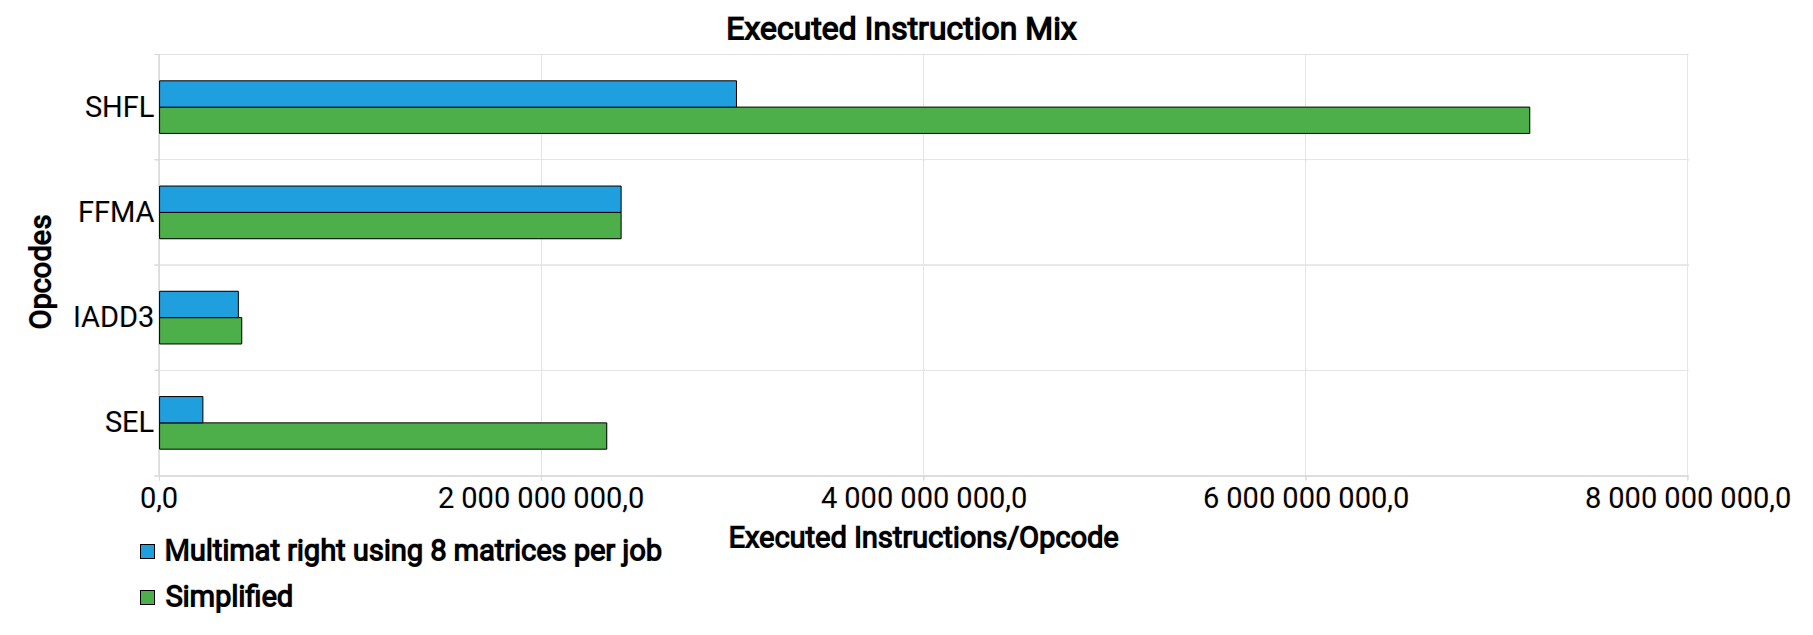
\includegraphics[width=\textwidth]{executed_instructions_multimat_right.png}
		\caption{Executed instruction mix.}
		\label{fig:executed_instructions_multimat_right}
	\end{subfigure}
	\hfill
	\begin{subfigure}{\textwidth}
		\centering
		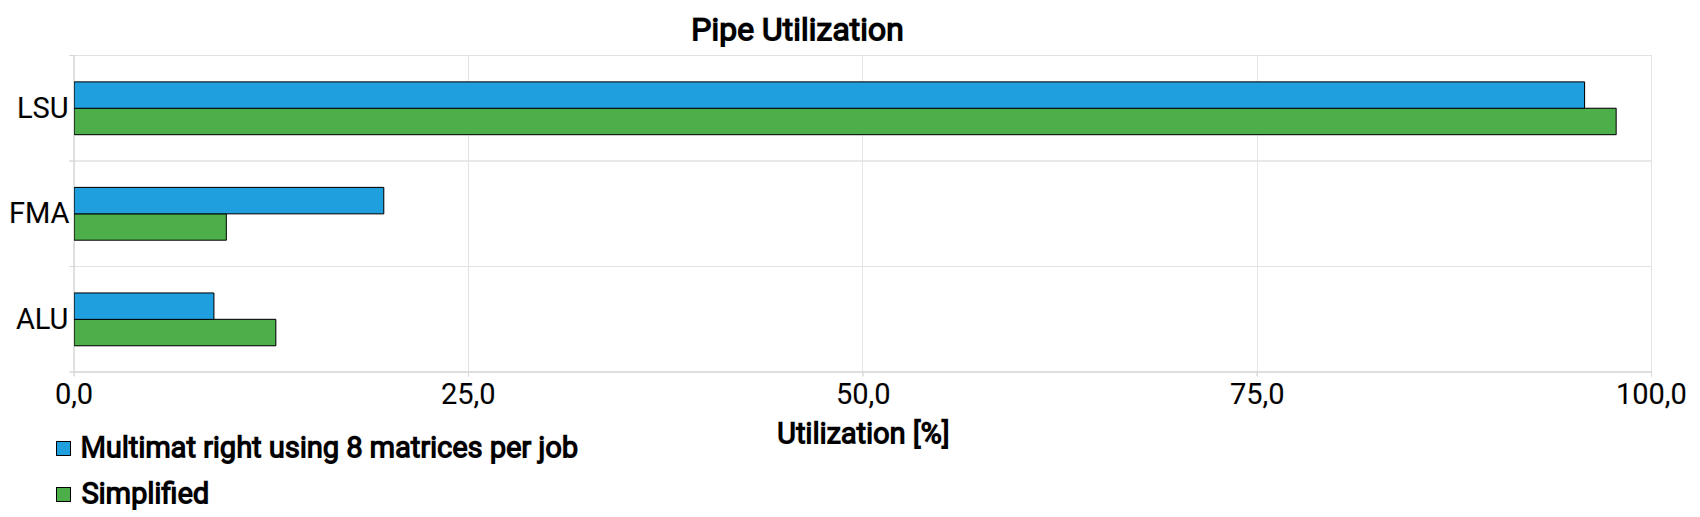
\includegraphics[width=\textwidth]{pipeline_utilization_multimat_right.png}
		\caption{Pipeline utilization.}
		\label{fig:pipeline_utilization_multimat_right}
	\end{subfigure}
	
	\caption{Comparison of \textit{one-to-many} simplified algorithm with the multiple right matrix optimization.}
	\label{fig:multimat_right_profiling}
\end{figure}

There are several ways to improve the ratio of SHFL instructions to FFMA instructions. The one with simplest changes to the code of the simplified implementation is to utilize the \textit{one-to-many} type of computation, and let each worker compute cross-correlation between one left matrix and many right matrices at once, as described in section \ref{sec:data_reuse_overlap} under the name \textit{multimat}. We call this exact implementation usable for \textit{one-to-many} and \textit{n-to-mn} types the \textit{multimat\_right} optimization, as each job contains multiple overlaps of a single left matrix with multiple right matrices. The obvious advantage is data reuse, as the data from the left matrix is used to compute multiple results. The main advantage is that each additional right matrix only adds a single SHFL instruction, while also adding one FFMA instruction. The ratio of SHFL to FFMA instructions can then be expressed as $2 + r : r$, where $r$ is the number of overlaps (from $r$ right matrices) computed by each worker, which for any value greater than $1$ is much improved from the $3:1$ ratio of the simplified warp shuffle algorithm.


The code changes required to implement this are very straight forward. As each job contains the same overlap between one left matrix and multiple right matrices, the three for loops and their bounds described in Section \ref{sec:simplified_warp_shuffle_steps} are left unchanged. The main difference is that the \textit{sum} and the \textit{thread\_right} variables in each thread are changed into arrays, utilizing the CUDA local array optimization described in Section \ref{sec:local_array_optimization}, as shown in the following snippet:

\begin{lstlisting}[
style=cuda
]
template<size_t NUM_RIGHTS, typename T>
__device__ void warp_shuffle_multimat_right_impl(...) {
	...
	T sum[NUM_RIGHTS];
	for (size_t r = 0; r < NUM_RIGHTS; ++r) {
		sum[r] = 0;
	}
	...
	T thread_right[NUM_RIGHTS];
	for (size_t r = 0; r < NUM_RIGHTS; ++r) {
		thread_right[r] = load_with_bounds_check(...);
	}
	...
	for (dsize_t r = 0; r < NUM_RIGHTS; ++r) {
		// Broadcast right buffer
		auto right_val = warp.shfl(thread_right[r], i);
		sum[r] += thread_left_bottom * right_val;
	}
}
\end{lstlisting}

We introduce the term \textit{matrix group}, describing the right input matrices from which overlaps are grouped into a single job. As the size of the matrix group must be known at compile time to utilize the CUDA local array optimization, we need to replicate the \textit{device} function implementing the algorithm for each supported matrix group size. This introduces a trade-off between compilation time, generated code size and the number of required registers on one hand and possible gains during run-time on the other. The actual matrix group size used during run-time is specified as run-time argument for the algorithm, which then chooses the correct implementation. If the number of matrices is not divisible by the matrix group size, the last few matrices will form a smaller matrix group which will choose the implementation based on its size. The maximum supported matrix group size is configurable during compile-time.


As with the simplified algorithm, thread block size is fixed to warp size in the \textit{x} axis and configurable by a run-time argument in the \textit{y} axis. The grid is then extended, this time in the \textit{x} axis (to allow simple combination with work distribution) to cover one output matrix from each matrix group. For each of these output matrices, there might be redundant workers due to the fixed size of thread block. These workers are handled the same way as in the simplified algorithm, by not writing to any output matrix or being stopped immediately if whole warp is redundant.
Due to the \textit{x} component of the thread block size set to warp size, there will not be a redundant warp due to grid extension, but there may still be redundant warps due to the fixed thread block size in the \textit{y} axis as in the simplified implementation.
 
Thanks to separately covering each output matrix, all threads of each thread block are always assigned overlaps from the same matrix group, which allows for reuse of much of the simplified algorithm code.

The effects of this optimization shown in Figure \ref{fig:multimat_right_profiling}, which compares the simplified algorithm against the optimized algorithm using 8 right matrices (default maximum group size due to compile times) per worker on input of size 256x256 with 1 left matrix and 16 right matrices, which are enough to saturate the RTX 2060 used for profiling. As we can see, the \texttt{LSU} pipeline is still a bottleneck even for the optimized algorithm, but the utilization of the \texttt{FMA} pipeline, which does the useful part of the computation, has increased from 9\% to 20\%. The most visible change is in the mix of the executed instructions, where we see a very noticeable improvement in the ratio of shuffle instructions (SHFL) to the floating point fused multiply-add instructions (FFMA). As expected, the ratio improves from $3 : 1$ to $10 : 8$. The small improvement in the \texttt{LSU} pipeline utilization can be explained by the comparatively low throughput of the SHFL instructions compared to the FFMA instructions. This is exacerbated by our use of Compute Capability 7.5 card for profiling, which has half the warp shuffle throughput of all other Compute Capabilities.

% TODO: Benchmark on gpulab
% TODO: Benchmark results

\subsection{Multiple rows from the right matrix}
\label{sec:multirow_right}

Another way to improve the instruction ratio is to process multiple overlaps from the same output matrix, which can be used even for the \textit{one-to-one} type of computation. We call this the \textit{multirow\_right} optimization based on how rows of the input matrices are loaded and processed. With this optimization, multiple consecutive overlaps from multiple rows of a single column of the output matrix are grouped into a single job. This is illustrated in Figure \ref{fig:multirow_shifts}, where we see two different jobs, each containing 4 overlaps, i.e. \textit{job\_size} is 4. 

\begin{figure}[ht]
	\centering
	\def\svgwidth{0.5\textwidth}
	\fontsize{6}{8}\selectfont
	% Must be relative to current directory
	% as input ignores graphicspath, which is
	% only for includegraphics{}
	\input{./img/overlap-Multirow.pdf_tex}
	\caption{Overlaps grouped into two different jobs by the \textit{multirow\_right} algorithm with 4 overlaps per job.}
	\label{fig:multirow_shifts}
\end{figure}

The core of the implementation is similar to the simplified algorithm. We compute the warp submatrix of the right input matrix containing all elements used by any of the overlaps in jobs assigned to the threads in the given warp. We then iterate over this submatrix, computing all \textit{job\_size} overlaps in a single pass. This reduces parallelism, as simplified algorithm would have split these overlaps into different jobs and computed them in parallel, but allows for data reuse, which is advantageous when the GPU is already saturated.

As each overlap in a given job has different shift in the \textit{y} axis, each overlap will contain different number of rows as shown in Figure \ref{fig:multirow_shifts}, but thanks to the column-wise grouping of overlaps, corresponding overlaps in each job assigned to threads of a single warp will contain the same group of rows. This again allows us to reuse much of the simplified implementation code, which expects a warp to process overlaps with the same number of rows.

Due to the different shifts of the overlaps in the \textit{y} axis, first $0$ to $job\_size - 1$ and last $0$ to $job\_size - 1$ rows of the warp submatrix may not be used for all $job\_size$ overlaps. Because of this, we must separate first few and last few iterations of the outer loop over rows of the warp submatrix into what we call \textit{Init} and \textit{Finish} iterations, illustrated in Figure \ref{fig:multirow_right_steps}. Overlaps in each job will always result in exactly $job\_size - 1$ steps split between Init and Finish steps depending on the exact overlap grouping.

Jobs containing overlaps with positive \textit{y} axis shift, as shown in Figure \ref{fig:multirow_init}, require Init steps. Jobs containing overlaps with negative \textit{y} axis shift, as show in Figure \ref{fig:multirow_fini}, require Finish steps. Jobs spanning shift $0$ on the \textit{y} axis require both Init and Finish steps.


Code changes for this implementation start similarly to changes for \textit{multimat\_right} from Section \ref{sec:multimat_right}. We again change the \textit{sum} and \textit{thread\_right} variables into arrays, utilizing the Local array optimization described in Section \ref{sec:local_array_optimization}. For this, we require that the number of overlaps grouped into a job, and consequently the number of rows loaded into the \textit{thread\_right} buffer, be known at compile time.


The three loops, the outer over rows of the warp submatrix, the middle over columns of the submatrix and the core loop over threads of the warp are separated. The middle and core loops are moved into a separate \textit{device} function named \textit{compute\_row\_group}, as they need to be reused for the Init, Finish and Main loop parts with different number of overlaps in each. The \textit{compute\_row\_group} is one of the functions that needs to be generated for each allowed value of \textit{job\_size}, as that determines the maximum number of overlaps grouped into a job, which corresponds to the maximum number of rows processed in a single iteration, be it Init, Finish or Main loop iteration. 

As described above, the outer loop is split into the three parts. There are always $job\_size - 1$ Init calls generated before the Main loop, where each Init call checks if the job assigned to the current thread contains overlaps with shifts requiring the given Init step. If required, Init step then calls \textit{compute\_row\_group} with the required number of overlaps, as shown in Figure \ref{fig:multirow_init} with Init 1 calling \textit{compute\_row\_group} for 1 overlap and Init 2 calling \textit{compute\_row\_group} for 2 overlaps. Main loop then goes through the warp matrix row by row, calling \textit{compute\_row\_group} each time on \textit{job\_size} overlaps. Finish steps then again always check if they are required before potentially calling \textit{compute\_row\_group} with the required number of overlaps.




\begin{figure}[ht]
	\centering	
	\begin{subfigure}{\textwidth}
		\centering
		\def\svgwidth{\textwidth}
		% Must be relative to current directory
		% as input ignores graphicspath, which is
		% only for includegraphics{}
		\input{./img/overlap-MultirowInit.pdf_tex}
		\caption{Complete computation of the \textit{multirow\_right} algorithm with \textit{job\_size} 3 for overlaps with shifts $[1, 1], [1, 2], [1, 3]$ showcasing Init steps.}
		\label{fig:multirow_init}
	\end{subfigure}
	\hfill
	\begin{subfigure}{\textwidth}
		\centering
		\def\svgwidth{\textwidth}
		% Must be relative to current directory
		% as input ignores graphicspath, which is
		% only for includegraphics{}
		\input{./img/overlap-MultirowFinalize.pdf_tex}
		\caption{Complete computation of the \textit{multirow\_right} algorithm with \textit{job\_size} 3 for overlaps with shifts $[1, -3], [1, -2], [1, -1]$ showcasing Finish steps}
		\label{fig:multirow_fini}
	\end{subfigure}
	
	\caption{Illustration of Init and Finish steps of the \textit{multirow\_right} algorithm with overlaps processed in each step displayed above the step.}
	\label{fig:multirow_right_steps}
\end{figure}



One of the disadvantages of this algorithm is the repeated reading of right input matrix rows by each worker. As warp shuffle is already utilized for data reuse in the given row, there is no simple mechanism to reuse data between rows as we traverse the warp submatrix from top to bottom. With 3 overlaps grouped into a job, each row of the right input matrix processed by the main loop is read 3 times by the worker, once for each of the overlaps assigned to the worker. Each time, it is used with different left row. This can be improved by also utilizing multiple rows from the left input matrix, computing multiple iterations of the current main loop at once. This implementation, named \textit{multirow\_both} as we read multiple rows in each iteration from both input matrices, is described in Section \ref{sec:multirow_both}.


When profiling this optimization, as shown in Figure \ref{fig:multirow_right_profiling}, we see similar improvements as with the previous \textit{multimat\_right} optimization. We have to keep in mind that the \textit{multirow\_right} algorithm improves the \textit{one-to-one} type of computation, which cannot be improved by the previous optimization. These two optimizations can also be combined, which is described in Section \ref{sec:combining_optimizations}. As before, the \textit{LSU} pipeline remains a bottleneck, but the utilization of \textit{FMA} pipeline is improved from 9\% to 17\%. With 4 overlaps per job, the ratio improves from $3 : 1$ to $6 : 4$ as expected from the $2 + r : r$ theoretical ratio. As this optimization improves the \textit{one-to-one} computation, it is more sensitive to occupancy reduction when workers process more than one overlap, mainly due to the smaller input size compared to the \textit{one-to-many} computation.

\begin{figure}[ht]
	\centering	
	\begin{subfigure}{\textwidth}
		\centering
		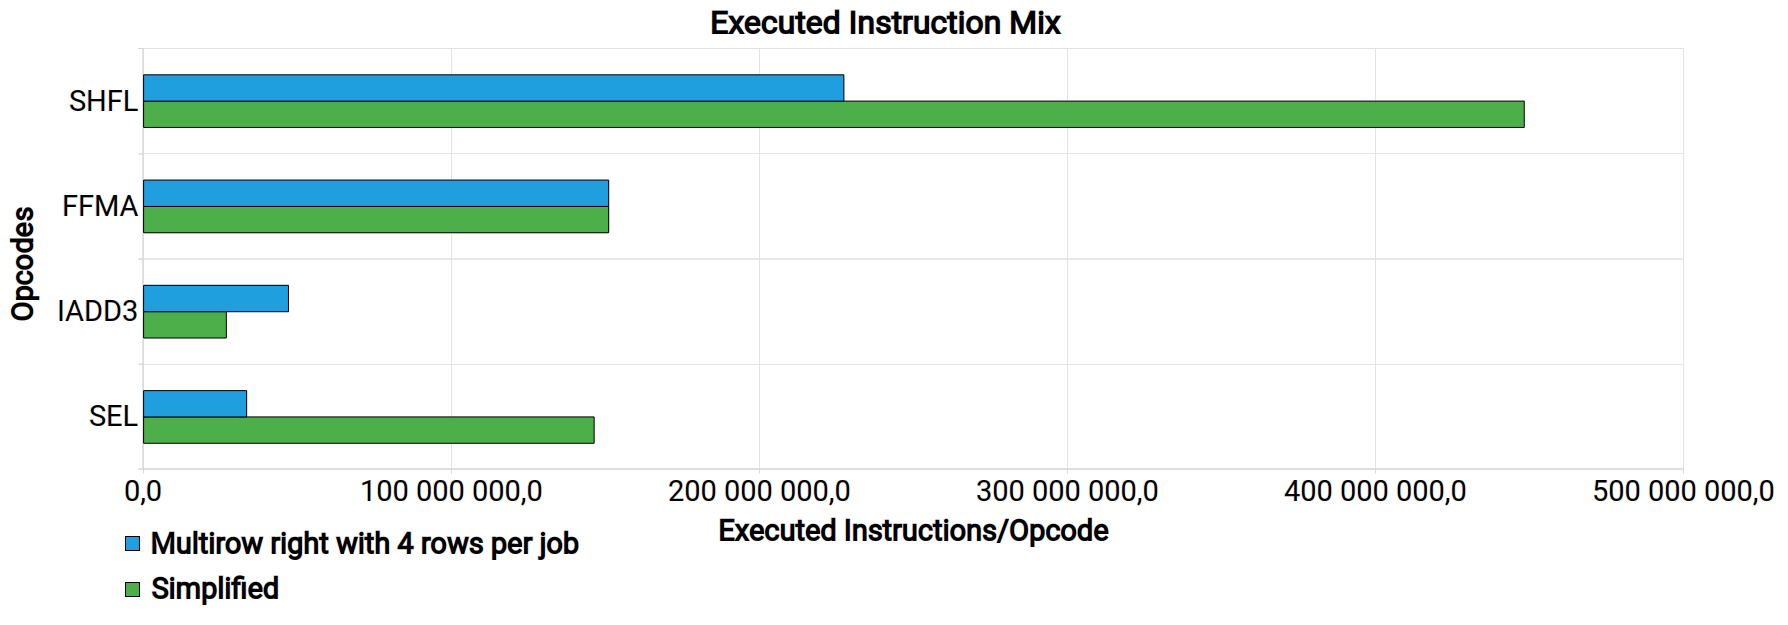
\includegraphics[width=\textwidth]{executed_instructions_multirow_right.png}
		\label{fig:executed_instructions_multirow_right}
	\end{subfigure}
	\hfill
	\begin{subfigure}{\textwidth}
		\centering
		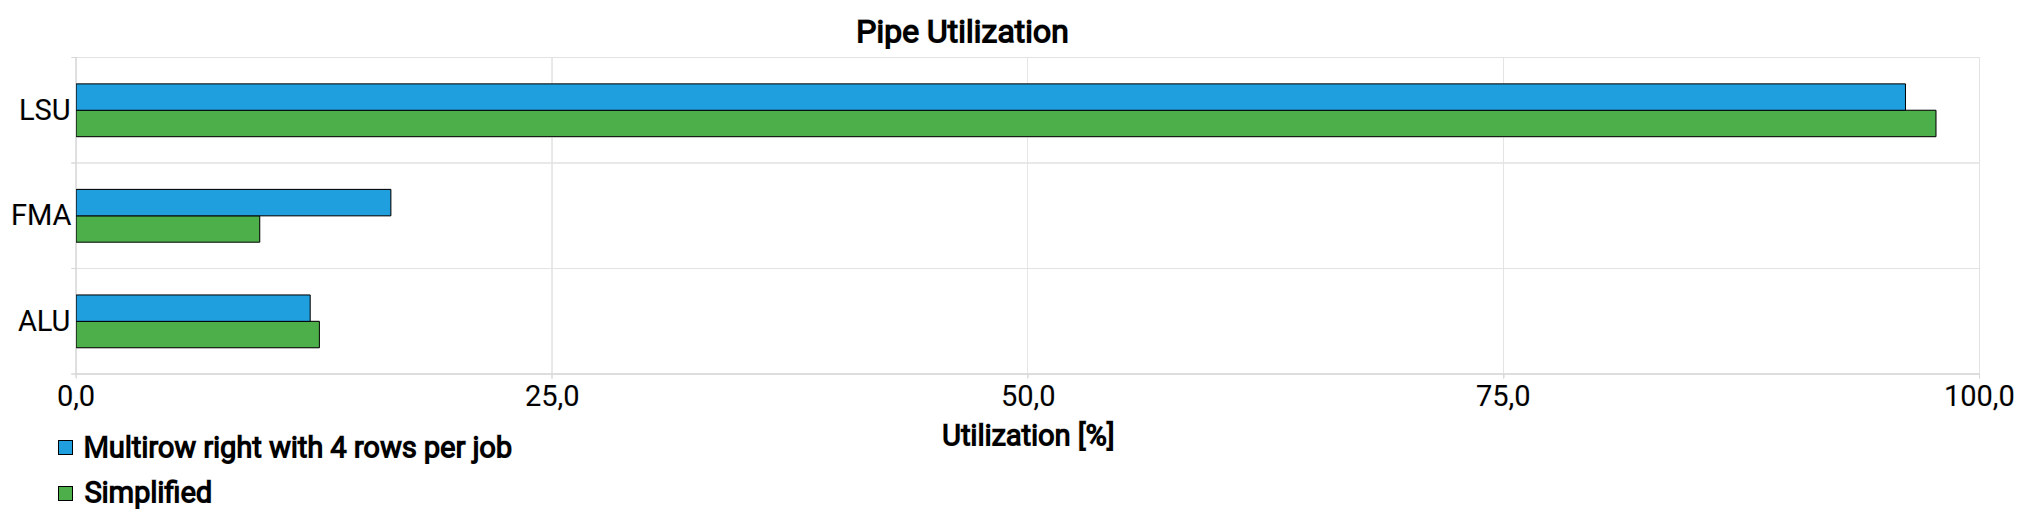
\includegraphics[width=\textwidth]{pipeline_utilization_multirow_right.png}
		\label{fig:pipeline_utilization_multirow_right}
	\end{subfigure}
	
	\caption{Comparison of \textit{one-to-one} simplified algorithm with the \textit{multirow\_right} optimization.}
	\label{fig:multirow_right_profiling}
\end{figure}

% TODO: Computing with double

% https://forums.developer.nvidia.com/t/loop-through-register-array-without-using-local-memory/29458/3
\section{Advanced warp shuffle optimizations}

The optimizations of the warp shuffle algorithm described up to this point hint at further possibilities, such as:
\begin{itemize}
	\item extending \textit{multimat\_right} optimization to also use multiple left matrices, creating \textit{multimat\_both} optimization;
	\item extending \textit{multirow\_right} to also use multiple rows from the left matrix, creating \textit{multirow\_both},
	\item combining several optimizations.
\end{itemize}

This section first illustrates problems we encountered with the Local array optimization, introduced in Section \ref{sec:local_array_optimization}, when implementing the \textit{multimat\_both} and \textit{multirow\_both} optimizations.
We then describe our solution to this problem, demonstrating the effects of this solution on the performance of the two advanced optimizations. We then present the details of \textit{multimat\_both} and \textit{multirow\_both} implementation, which extend the basic optimizations described in Section \ref{sec:warp_shuffle_alg}. Lastly we combine all the basic and advanced optimizations together, creating the final implementation of the warp shuffle algorithm. 

\subsection{Advanced optimizations and local arrays}
\label{sec:local_array_optimization_code_changes}

When implementing the \textit{multimat\_both} and \textit{multirow\_both} optimizations, described in detail in the following sections \ref{sec:multimat_both} and \ref{sec:multirow_both} respectively, we encountered a problem with the \textit{nvcc} compiler not optimizing the local arrays into registers. 

Using profiling and examining the SASS, we isolated the problem to the \textit{thread\_left\_bottom} and \textit{thread\_left\_top} arrays. We further isolated it to the following part of the code, which in its original form shared by the simplified, \textit{multimat\_right} and \textit{multirow\_right} implementations looks like this:

\begin{lstlisting}[
style=cuda
]
thread_left_bottom = warp.shfl(
	warp.thread_rank() != 0 ? thread_left_bottom : thread_left_top,
	warp.thread_rank() + 1
);
thread_left_top = warp.shfl_down(thread_left_top, 1);
\end{lstlisting}

To process multiple values from left input matrices, which is the basis of both \textit{multimat\_both} and \textit{multirow\_both} optimizations, the code needs to be changed into the following:

\begin{lstlisting}[
style=cuda
]
#pragma unroll
for (size_t l = 0; l < NUM_LEFTS; ++l) {
	thread_left_bottom[l] = warp.shfl(
		warp.thread_rank() != 0 ? thread_left_bottom[l] : thread_left_top[l],
		warp.thread_rank() + 1
	);
	thread_left_top[l] = warp.shfl_down(thread_left_top[l], 1);
}
\end{lstlisting}

The \textit{nvcc} compiler should be able to unroll this loop, and thanks to static indexing, the \textit{thread\_left\_bottom} and \textit{thread\_left\_top} local arrays should be optimized into registers. Unfortunately, as we can see in Listing \ref{lst:sass_local_mem}, the compiler behaves as if dynamic indexing was used and pushes the arrays into local memory. 
Due to the closed source nature of the \textit{nvcc} compiler, we can only speculate on the reasons why the loop unrolling does not result in static indexing. One possibility, based on the generated SASS instructions seen in Listing \ref{lst:sass_local_mem}, is that the ternary operator is optimized into dynamic array indexing, which then prevents the local array optimization. As there is no visible branching in the unrolled loop, the base address of either the \textit{thread\_left\_bottom} or the \textit{thread\_left\_top} is loaded into register R63, which is then reused in all loads, resulting in dynamic indexing. 

% TODO: Add coloring
\begin{lstlisting}[
style=sass,
caption={SASS instructions without local array optimization},
label=lst:sass_local_mem
]
LDL R0, [R63+0x4]
SHFL.IDX PT, R8, R0, R57, 0x1f
SHFL.DOWN PT, R0, R32, 0x1, 0x1f
STL [R62], R8
STL [R61], R0
\end{lstlisting}

We experimented with several solutions, with the following version compiling into static indexing:

\begin{lstlisting}[
style=cuda
]
#pragma unroll
for (size_t l = 0; l < NUM_LEFTS; ++l) {
	T bottom_shift_val;
	if (warp.thread_rank() != 0) {
		bottom_shift_val = thread_left_bottom[l];
	} else {
		bottom_shift_val = thread_left_top[l];
	}

	thread_left_bottom[l] = warp.shfl(bottom_shift_val, warp.thread_rank() + 1);
	thread_left_top[l] = warp.shfl_down(thread_left_top[l], 1);
}
\end{lstlisting}

% TODO: Add coloring
\begin{lstlisting}[
style=sass,
caption={SASS instructions with local array optimization},
label=lst:sass_no_local_memory
]
SEL R42, R52, R20, !P4
SHFL.IDX PT, R53, R48, R53, 0x1f
SHFL.DOWN PT, R52, R52, 0x1, 0x1f
\end{lstlisting}

The only change is the expansion of the ternary operator into an equivalent if statement. As shown in Listing \ref{lst:sass_no_local_memory}, the body of the updated loop results in a single \textit{SEL} instruction which selects the top or the bottom part of the buffer. This version of the loop is used by the advanced warp shuffle optimizations described in the following sections.

The difference is also visible in Figure \ref{fig:instruction_mix_local_mem}, which shows the additional local memory store (STL) and load (LDL) instructions in both the \textit{multimat\_both} and \textit{multirow\_both} without local array optimization. Apart from these additional instructions, the number of remaining instructions is generally the same, with some additional integer multiply-add instructions (IMAD) in Figure \ref{fig:shuffle_multirow_both_instruction_mix} due to local memory address computations.

\begin{figure}[ht]
	\centering	
	\begin{subfigure}{\textwidth}
		\centering
		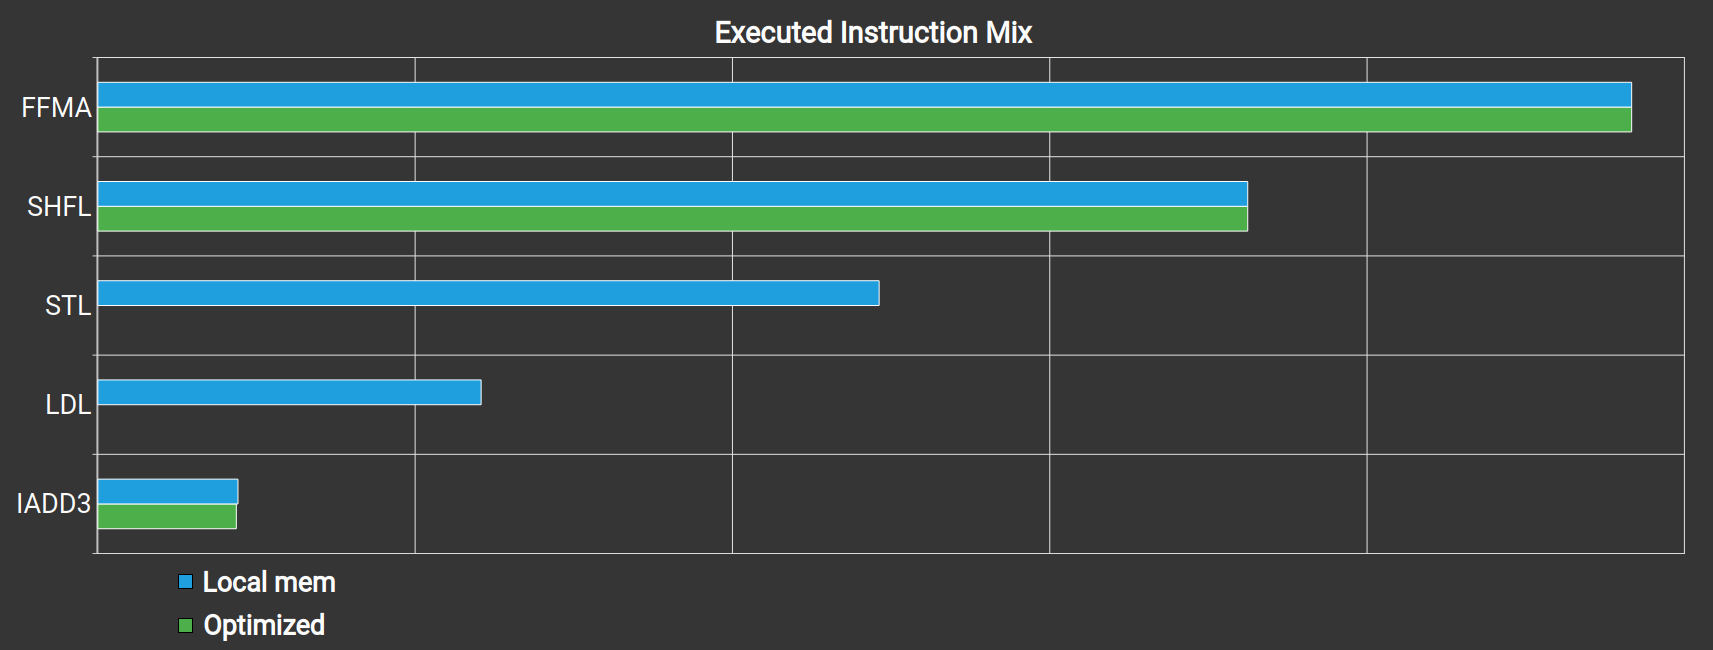
\includegraphics[width=0.7\textwidth]{executed_instructions_shuffle_multimat_both.png}
		\caption{The \textit{multimat\_both} optimization.}
		\label{fig:shuffle_multimat_both_instruction_mix}
	\end{subfigure}
	\hfill
	\begin{subfigure}{\textwidth}
		\centering
		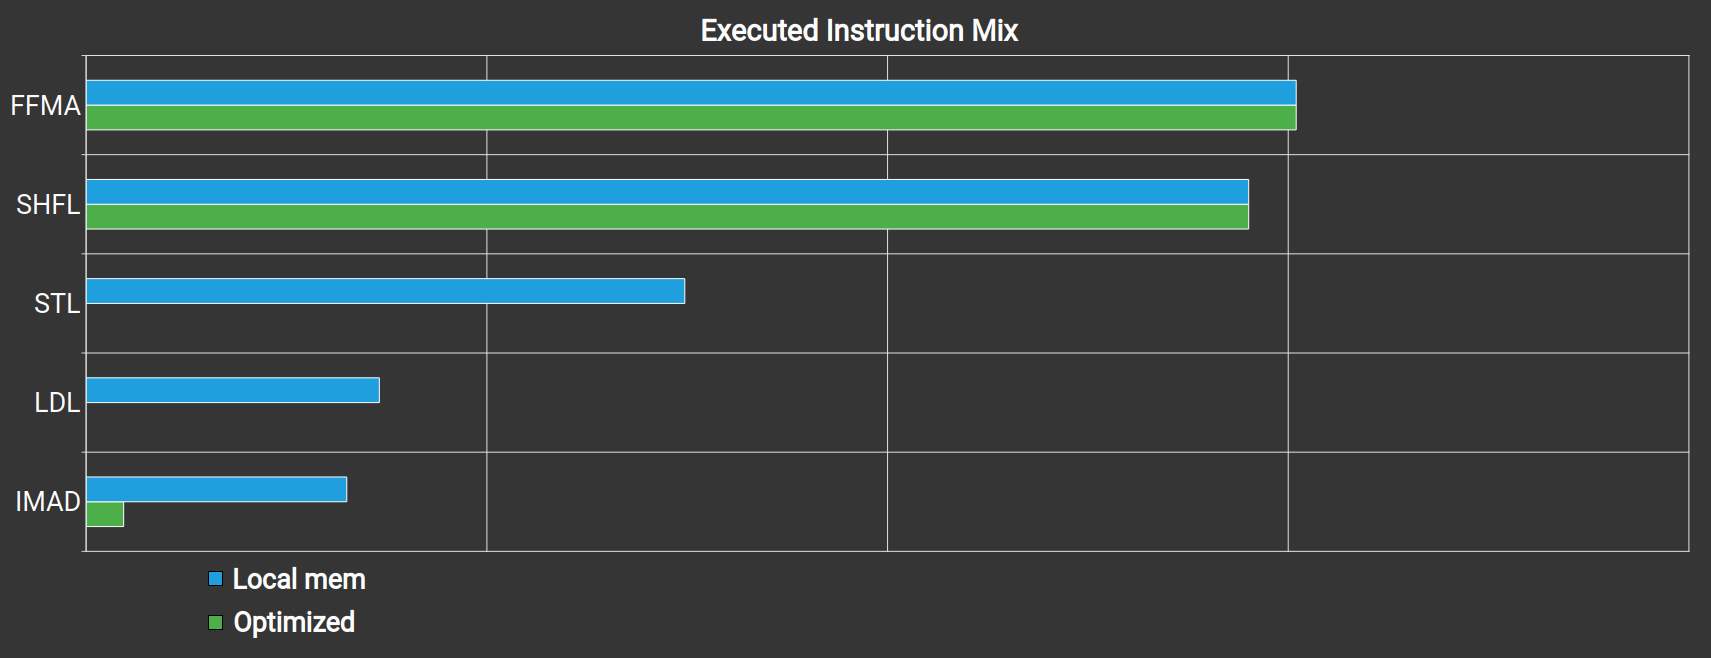
\includegraphics[width=0.7\textwidth]{executed_instructions_shuffle_multirow_both.png}
		\caption{The \textit{multirow\_both} optimization.}
		\label{fig:shuffle_multirow_both_instruction_mix}
	\end{subfigure}
	
	\caption{Comparison of the instruction mix between a version with arrays in local memory and a version with arrays in registers.}
	\label{fig:instruction_mix_local_mem}
\end{figure}

Based on this observation, the measured speedup in Figure \ref{fig:speedup_local_mem} is caused solely by the application of the local array optimization. The speedup for smaller inputs is limited due to low occupancy, but is still present. As an example, Figure \ref{fig:multimat_both_speedup} shows that for input matrices of size 64 by 64, the solution without local memory access is already 2 times faster. Figure \ref{fig:multirow_both_speedup} shows that there is slightly smaller improvement in the \textit{multirow\_both} optimization compared to the \textit{multimat\_both}. This is most likely caused by higher general overhead due to the greater overall complexity of the optimization.


\begin{figure}[ht]
	\centering	
	\begin{subfigure}{0.45\textwidth}
		\centering
		\def\svgwidth{\textwidth}
		% Must be relative to current directory
		% as input ignores graphicspath, which is
		% only for includegraphics{}
		\input{./img/multimat_speedup.pdf_tex}
		\caption{The \textit{multimat\_both} optimization.}
		\label{fig:multimat_both_speedup}
	\end{subfigure}
	\hfill
	\begin{subfigure}{0.45\textwidth}
		\centering
		\def\svgwidth{\textwidth}
		% Must be relative to current directory
		% as input ignores graphicspath, which is
		% only for includegraphics{}
		\input{./img/multirow_speedup.pdf_tex}
		\caption{The \textit{multirow\_both} optimization.}
		\label{fig:multirow_both_speedup}
	\end{subfigure}
	
	\caption{Improvement of the two optimizations without local memory access.}
	\label{fig:speedup_local_mem}
\end{figure}


\subsection{Multiple left matrices}
\label{sec:multimat_both}

A natural step following the use of the same overlap of multiple right matrices is to also group the same overlaps between multiple left matrices and multiple right matrices into a single job, as described in Section \ref{sec:data_reuse_overlap}. This optimization is only usable for the \textit{n-to-m} computation type, as the \textit{n-to-mn} type correlates each left matrix with a different set of right matrices.

To implement this optimization, we start with the the code of the \textit{multimat\_right} optimization. We add additional template parameter \textit{NUM\_LEFTS} to the implementing function and change both \textit{thread\_left\_bottom} and \textit{thread\_left\_top} from simple variables into local arrays, as was done for the \textit{thread\_right} variable by the \textit{multimat\_right} optimization. The number of overlaps computed by each thread is also changed to $NUM_LEFTS * NUM_RIGHTS$ from only $NUM_RIGHTS$. The changes are illustrated by the following snipped: 

\begin{lstlisting}[
style=cuda
]
template<size_t NUM_RIGHTS, size_t NUM_LEFTS, typename T>
__device__ void warp_shuffle_multimat_both_impl(...) {
	...
	T sum[NUM_RIGHTS * NUM_LEFTS];
	for (size_t s = 0; s < NUM_RIGHTS; ++s) {
		sum[s] = 0;
	}
	...
	T thread_left_bottom[NUM_LEFTS];
	for (size_t l = 0; l < NUM_LEFTS; ++l) {
		thread_left_bottom[l] = load_with_bounds_check(...);
	}
	...
	T thread_left_top[NUM_LEFTS];
	for (size_t l = 0; l < NUM_LEFTS; ++l) {
		thread_left_top[l] = load_with_bounds_check(...);
	}
	...
	for (size_t r = 0; r < NUM_RIGHTS; ++r) {
		auto right_val = warp.shfl(thread_right[r], i);
		
		for (size_t l = 0; l < NUM_LEFTS; ++l) {
			sum[l * NUM_RIGHTS + r] += thread_left_bottom[l] * right_val;
		}
	}
	...
}
\end{lstlisting}

Similarly to the \textit{multimat\_right} optimization, we group input matrices into matrix groups, this time separately grouping left matrices into \textit{left\_matrix\_groups} and right matrices into \textit{right\_matrix\_groups}, where \textit{right\_matrix\_groups} are equivalent to the original matrix groups from the \textit{multimat\_right} optimization. The number of matrices in a left matrix group is configured independently of the number of matrices in a right matrix groups. As shown in the code snippet above, maximum size of left matrix group and right matrix group has to be known at compile time so that we can generate the \textit{warp\_shuffle\_multimat\_both\_impl} for all combinations of these values from 0 to the configured maximum. At run-time, the implementation chooses the correct method. The last matrix groups from both left and right input matrices may be smaller as the number of left or right matrices may not be divisible by the value of the run-time argument. The implementation then chooses the function with the correct matrix group size.

As with the simplified algorithm, the block size is set to warp size in the \textit{x} axis and configurable by run-time argument in the \textit{y} axis. 
When extending the grid, we require expansion in four axes. Two to cover a single output matrix, one for left matrix groups and one for right matrix groups. 
These four axes need to be compressed into a three dimensional grid. To achieve this, we use the \textit{x} axis to both cover columns of a single output matrix while also utilizing it to expand the grid across left matrix groups. The \textit{y} axis is used to expand grid over the right matrix groups. The last axis, \textit{z}, is used to cover the rows of the single output matrix . We choose to do this using the last grid axis to behave similar to the \textit{multimat\_right} and prepare the \textit{multimat\_both} optimization for combination with the work distribution optimization. 


% TODO: Redundant workers
% TODO: Separate covering of an output matrix from each group

This optimization improves the ratio of warp shuffle to fused multiply-add instructions to $ 2 * l + r : l * r$, where $l$ is the number of left matrices and $r$ the number of right matrices utilized by each worker. This results in a noticeable improvement in the executed instruction mix shown in Figure \ref{fig:shuffle_multimat_both_instruction_mix}. 


\subsection{Multiple rows from both matrices}
\label{sec:multirow_both}

When improving the \textit{one-to-one} computation using the \textit{multirow\_right} optimization described in Section \ref{sec:multirow_right}, which processes multiple overlaps from consecutive rows of a single column of the output matrix, we hinted at a further improvement using multiple rows from the left matrix in the main loop. This not only improves the ratio of warp shuffle to fused multiply-add instructions, but also reduces the number of times every row from the right input matrix is read. 

The main change is that the main loop now advances by multiple left input matrix rows instead of a single row. The exact number of left rows to advance by is configured using run-time argument. An additional stage between the multistep main loop and Finish is also needed to compute the remaining rows from the left input matrix when the total number of left input matrix rows is not divisible by the main loop step. This stage utilizes the original single step main loop. The Init and Finish parts are left unchanged.

The algorithm parameters are changed from just the number of right rows processed in each main loop iteration (which corresponds to the number of overlaps assigned to a single thread) to a pair of parameters, the number of left rows to process in each iteration of the main loop and the number of overlaps, also called shifts in the code, to be processed by each thread. The number of right rows to be loaded is now derived from the number of overlaps and the number of left rows. In each iteration of the main loop, the left row 0 is processed with right rows $[0, NUM\_SHIFTS - 1]$, left row 1 with right rows $[1, NUM\_SHIFTS]$ and left row \textit{l} with right rows $[l, NUM\_SHIFTS - 1 + l]$. This gives us the number of right rows to load, which is $NUM\_SHIFTS + NUM_LEFT_ROWS - 1$ so that we can process all the left rows simultaneously. 

The ratio of warp shuffle instructions (SHFL) to fused multiply-add instructions (FFMA) for this optimization is $l + (s - 1 + l) : l * s$ in the main loop, where $l$ is the number of left rows processed by each iteration of the main loop and $s$ is the number of shifts processed by each thread.  
The Init, single step main loop and Finish parts share the original ratio of the \textit{multirow\_right} implementation. This ratio is also apparent in Figure \ref{fig:shuffle_multirow_both_instruction_mix}.


\subsection{Combining the optimizations}
\label{sec:combining_optimizations}

We have implemented the following optimizations of the Warp Shuffle algorithm:

\begin{itemize}
	\item work distribution,
	\item \textit{multimat\_right},
	\item \textit{multirow\_right},
	\item \textit{multimat\_both},
	\item \textit{multirow\_both}.
\end{itemize}

As described in Sections \ref{sec:multimat_both} and \ref{sec:multirow_both}, the  \textit{multimat\_both} and \textit{multirow\_both} optimizations are implemented as extensions to the \textit{multimat\_right} and \textit{multirow\_right} optimizations respectively.


All of the optimizations listed above can be combined with the following restrictions:

\begin{enumerate}
	\item \textit{multirow} optimizations cannot be combined with work distribution,
	\item \textit{multimat\_both} can only be used to optimize the \textit{n\_to\_m} computation. 
\end{enumerate}

With the \textit{multirow} optimization, each job contains several different overlaps of the two input matrices, where each overlap has different number of rows. As our work distribution optimization is based on the number of rows of the overlap, the current implementation cannot be easily reused. This is not a problem with the \textit{multimat} optimizations, in which each thread computes the same overlap in multiple output matrices.

The \textit{n\_to\_m} computation type is the only type where multiple left matrices share the same right matrix, which makes it possible to reuse the data from the left matrices.


With these restrictions in mind, we have implemented the following versions of the warp shuffle algorithm:

% TODO: Maybe change into a table with matching implemented calculation types
\begin{itemize}
	\item multimat\_right,
	\item multimat\_right\_work\_distribution,
	\item multimat\_both\_work\_distribution,
	\item multirow\_right,
	\item multirow\_right\_multimat\_right,
	\item multirow\_both,
	\item multirow\_both\_multimat\_right,
	\item multirow\_both\_multimat\_both.
\end{itemize}

Both \textit{multimat} optimizations were already prepared for combination with work distribution, as hinted at in their respective sections. The core computation code does not change, the only difference is that we split the original warp submatrix the same way we did when implementing work distribution for simplified warp shuffle algorithm, described in Section \ref{sec:warp_shuffle_work_dist}. Each time we utilize the last used grid size axis to multiply the number of workers started. For \textit{multimat\_right}, it is the \textit{y} axis, for \textit{multimat\_both}, it is the \textit{z} axis.

Combination of \textit{multimat} and \textit{multirow} optimizations takes the implementation of \textit{multimat} optimization, separates the middle and inner loop as is done to the simplified implementation in the implementation of \textit{multirow} and splits the outer loop iterations into init, main loop, single step main loop, and finish parts.

These implementations are measured and compared in Section \ref{sec:results_warp_shuffle}.

\section{Occupancy improvement}
\label{sec:occupancy_improvements}

For small inputs, processing a single overlap or a row group per thread may not split the computation into enough jobs to saturate the whole GPU, leading to low occupancy. As described in Section \ref{sec:occupancy}, low occupancy prevents the GPU from hiding the high latency of each instruction, resulting in poor performance. To increase the number of threads started for smaller inputs, we increase the size of each worker from a single thread to a whole warp or even a whole thread block. This increase in number of threads in combination with the small input data size leads to a need of balancing the overhead of each thread with the reduced workload. The overhead consists mainly of scheduling, repeated data reads, and computation of array indexes for each access. 

%For each implementation, there exists an input size for which the overhead results in pure CPU based implementation being faster than the GPU implementation. This bound is specific to each system, as it is based on the relative power of the CPU and GPU, together with the interconnection between GPU and CPU for data transfer. This topic is further explored in Section \ref{sec:warp_per_shift_vs_cpu}.

In this section, we first introduce a simplified implementation of the \textit{warp per shift} algorithm utilizing whole warps as workers with each job containing a single overlap, also called shift. We then introduce several improvements of this algorithm, first by using shared memory and then by further increasing the number of jobs using work distribution optimization, adapted from the implementation described in Section \ref{sec:warp_shuffle_work_dist}. Lastly we implement an algorithm utilizing whole thread blocks as workers, again with each job containing a single overlap.

\subsection{Warp per shift}

Implementation of the \textit{Warp per shift} algorithm is very simple compared to the warp shuffle-based algorithm described in Section \ref{sec:warp_shuffle_alg}. The basic implementation utilizes whole warps as workers and assigns each worker a job consisting of a single overlap. Each overlap is uniquely identified by the shift of the two input matrices, and the shift is what is stored and propagated throughout the code. This is why we call this the \textit{warp per shift} algorithm.

\begin{figure}[ht]
	\centering	
	\begin{subfigure}{0.55\textwidth}
		\fontsize{6}{8}\selectfont
		\centering
		\def\svgwidth{\textwidth}
		% Must be relative to current directory
		% as input ignores graphicspath, which is
		% only for includegraphics{}
		\input{./img/overlap-Shifts.pdf_tex}
		\caption{Output matrix and the corresponding overlaps.}
		\label{fig:warp_per_shift_overlaps}
	\end{subfigure}
	\hfill
	\begin{subfigure}{0.4\textwidth}
		%\fontsize{6}{8}\selectfont
		\centering
		\def\svgwidth{\textwidth}
		\fontsize{6}{8}\selectfont
		% Must be relative to current directory
		% as input ignores graphicspath, which is
		% only for includegraphics{}
		\input{./img/overlap-WarpPerShiftWarps.pdf_tex}
		\caption{Distribution of overlaps in a 3 by 7 output matrix between thread blocks and their warps.}
		\label{fig:warp_per_shift_warps}
	\end{subfigure}
	
	\caption{Output matrix and its distribution between warps.}
\end{figure}

As in the Basic algorithm, introduced in Section \ref{sec:basic_alg}, this implementation uses two dimensional grid of two dimensional thread blocks to cover output matrix. The difference is in how we use each dimension to map threads to overlaps, this time based on which warp and thread block they are part of. All threads of a warp are assigned the same overlap and they cooperate to compute all the tasks (yellow boxes) which belong to this overlap. The mapping from thread blocks and warps to overlaps of the output matrix is illustrated by Figure \ref{fig:warp_per_shift_warps}. The \textit{x} axis of thread block size is again set to warp size to simplify grouping of threads to warps, with the \textit{y} axis again configurable using run-time argument. Warps of each thread block are assigned consecutive overlaps in a row of the output matrix using the \textit{y} component of thread block size, which determines the number of warps in each thread block. This means that each thread block is assigned \textit{y} overlaps in one of the output matrix rows.
The \textit{x} and \textit{y} components of grid size are then used to cover the matrix using these thread blocks.


Each thread of a warp is assigned subset of the multiplication tasks (yellow boxes), as shown in Figure \ref{fig:warp_per_shift_normal_indexing}, which it computes and holds the sum in local variable. This distribution is done using the following code:

\begin{lstlisting}[
style=cuda
]
for (
	size_t i = warp.thread_rank(); 
	i < total_items; 
	i += warp.size()
) {
	size_t overlap_row = i / overlap_size.x;
	size_t overlap_row_offset = i % overlap_size.x;

	size_t right_idx = ...;
	size_t left_idx = ...;

	sum += left[left_idx] * right[right_idx];
}
\end{lstlisting}

\begin{figure}[ht]
	\centering
	\def\svgwidth{0.2\textwidth}
	\fontsize{8}{10}\selectfont
	% Must be relative to current directory
	% as input ignores graphicspath, which is
	% only for includegraphics{}
	\input{./img/warp_per_shift-Basic.pdf_tex}
	\caption{Thread computing given task with basic indexing (example warp size 4).}
	\label{fig:warp_per_shift_normal_indexing}
\end{figure}

This distribution of tasks minimizes thread divergence but may lead to uncoalesced global memory access. Another possible disadvantage of this implementation is the division and the modulo instruction in each loop iteration, which is used to determine the position in the overlapping submatrix to be computed by the current thread.

The sums computed by each thread of the warp are then combined using the \texttt{cooperative\_groups::reduce} function, which may even be hardware accelerated if running on the newest Ampere GPUs. The final result is then written by thread with warp rank $0$ to the output matrix. 


\subsection{Simplified indexing}

The Simplified indexing is an attempt to solve the problems highlighted in the previous section, namely the uncoalesced global memory access and the low throughput division instruction in the main loop. To fix these problems, we change the distribution of tasks between threads as shown in Figure \ref{fig:warp_per_shift_simplified_indexing}. Compared to basic indexing described in the previous section, each row of the overlap is processed independently and fully before continuing to the next row. This assures coalesced access to the global memory, but leads to thread divergence if the row size of the overlap is not a multiple of warp size, as is the case in Figure \ref{fig:warp_per_shift_simplified_indexing}.

\begin{figure}[ht]
	\centering
	\def\svgwidth{0.5\textwidth}
	\fontsize{8}{10}\selectfont
	% Must be relative to current directory
	% as input ignores graphicspath, which is
	% only for includegraphics{}
	\input{./img/warp_per_shift-SimplifiedIndexing.pdf_tex}
	\caption{Comparison of task assignment with basic and simplified indexing (example warp size 4).}
	\label{fig:warp_per_shift_simplified_indexing}
\end{figure}

Thread divergence is the major problem of this implementation. Based on our profiling, the simplified indexing leads to an average of only 15.31 of the 32 threads executing each instruction and not being predicated (masked by a predicate). With basic indexing on the same hardware, this average improves to 26.85, which is almost twice the work done per instruction. The main reason for this difference is shown in Figure \ref{fig:warp_per_shift_thread_divergence}. This figure shows the worst case scenario, where simplified indexing leads to the rows being processed sequentially, whereas basic indexing executes this in a single iteration. Overlaps such as this make up a sizable part of every cross-correlation computation. Because of this, simplified indexing does not improve execution times.

\begin{figure}[ht]
	\centering
	\def\svgwidth{0.45\textwidth}
	\fontsize{8}{10}\selectfont
	% Must be relative to current directory
	% as input ignores graphicspath, which is
	% only for includegraphics{}
	\input{./img/warp_per_shift-ThreadDivergence.pdf_tex}
	\caption{Task assignment with basic and simplified indexing to showcase thread divergence when using simplified indexing.}
	\label{fig:warp_per_shift_thread_divergence}
\end{figure}

Even though simplified indexing should theoretically lead to better coalescing of global memory access, the opposite seems to be the case as illustrated by Figure \ref{fig:executed_instructions_simplified_indexing}. This may be highly dependent on Compute Capability of the underlying hardware, but on CC 7.5 of RTX 2060, we observe a 47\% increase in the number of global memory requests when using simplified indexing. This corresponds to high \textit{LSU} pipeline usage of 88\% visible in Figure \ref{fig:pipeline_utilization_simplified_indexing}, which becomes a bottleneck. The profiling was done on input matrices of size 64 by 64 containing 32bit floating point numbers. In these matrices, each row is 256B in size. In many overlaps, the last item of each row will be less than 128B (global memory transaction size) from the first item in the next row. This leads to coalescing of the global memory read with basic indexing but results in 2 separate accesses with simplified indexing. This may explain the 47\% difference in global memory requests.

Another visible difference in Figure \ref{fig:executed_instructions_simplified_indexing} is the increase in number of instructions across the board, most visible with branching (BRA) and barrier synchronization (BSYNC) instructions. This is caused by the increase in number of iterations each warp executes to process the same data. Even with the increase in number of instructions, the \textit{ALU} and \textit{FMA} pipelines are less utilized than with basic indexing. This is caused by warps waiting for warp recombination on the barrier synchronization points and loads from global memory.


\begin{figure}[ht]
	\centering	
	\begin{subfigure}{0.8\textwidth}
		\centering
		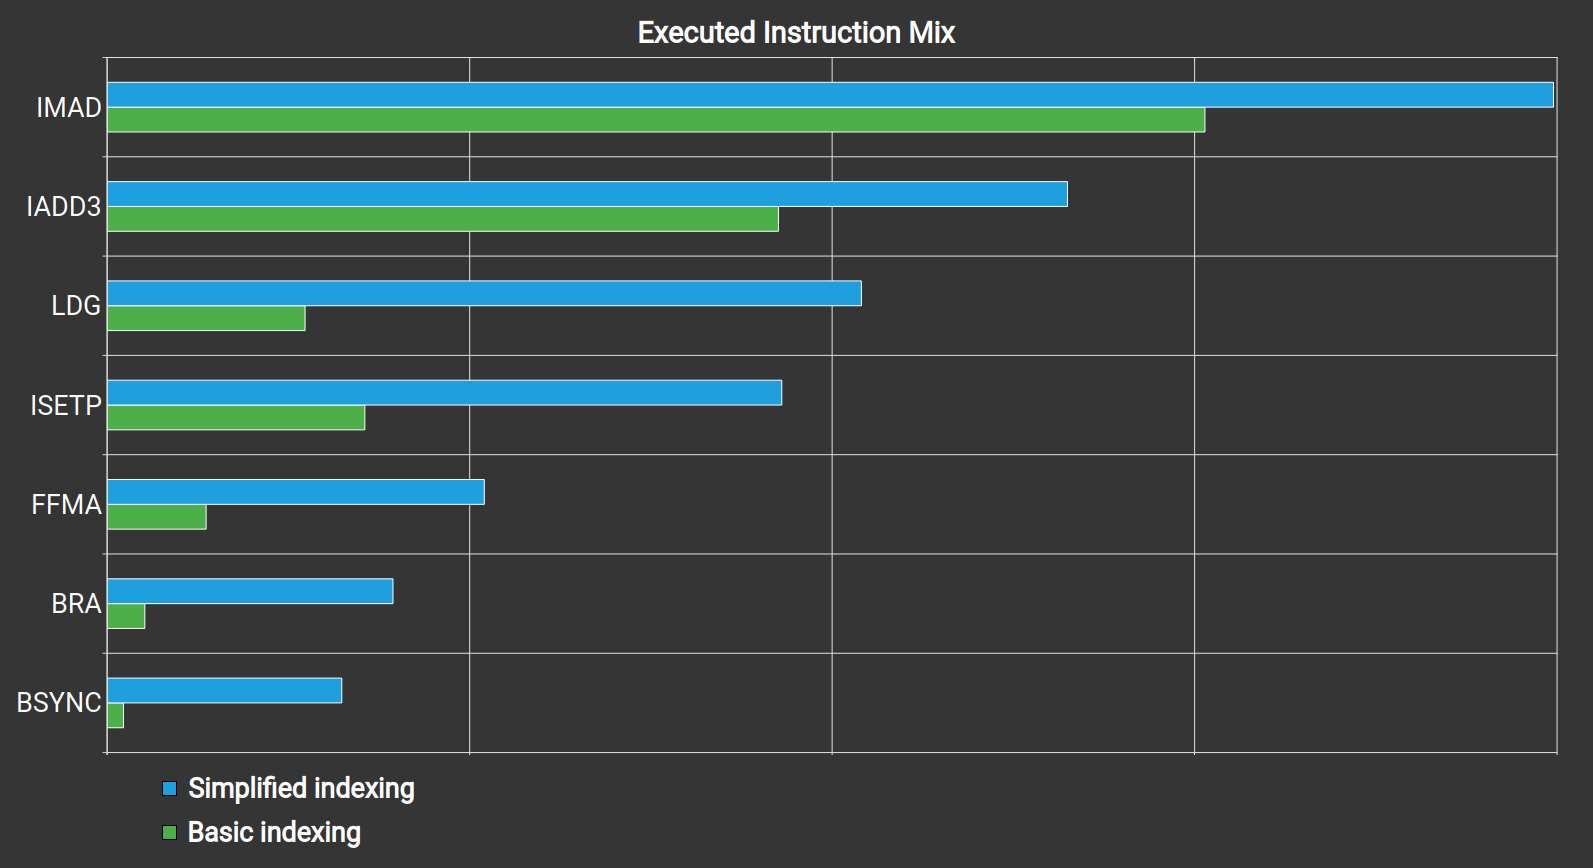
\includegraphics[width=\textwidth]{executed_instructions_simplified_indexing.png}
		\caption{Executed instruction mix.}
		\label{fig:executed_instructions_simplified_indexing}
	\end{subfigure}
	\hfill
	\begin{subfigure}{0.8\textwidth}
		\centering
		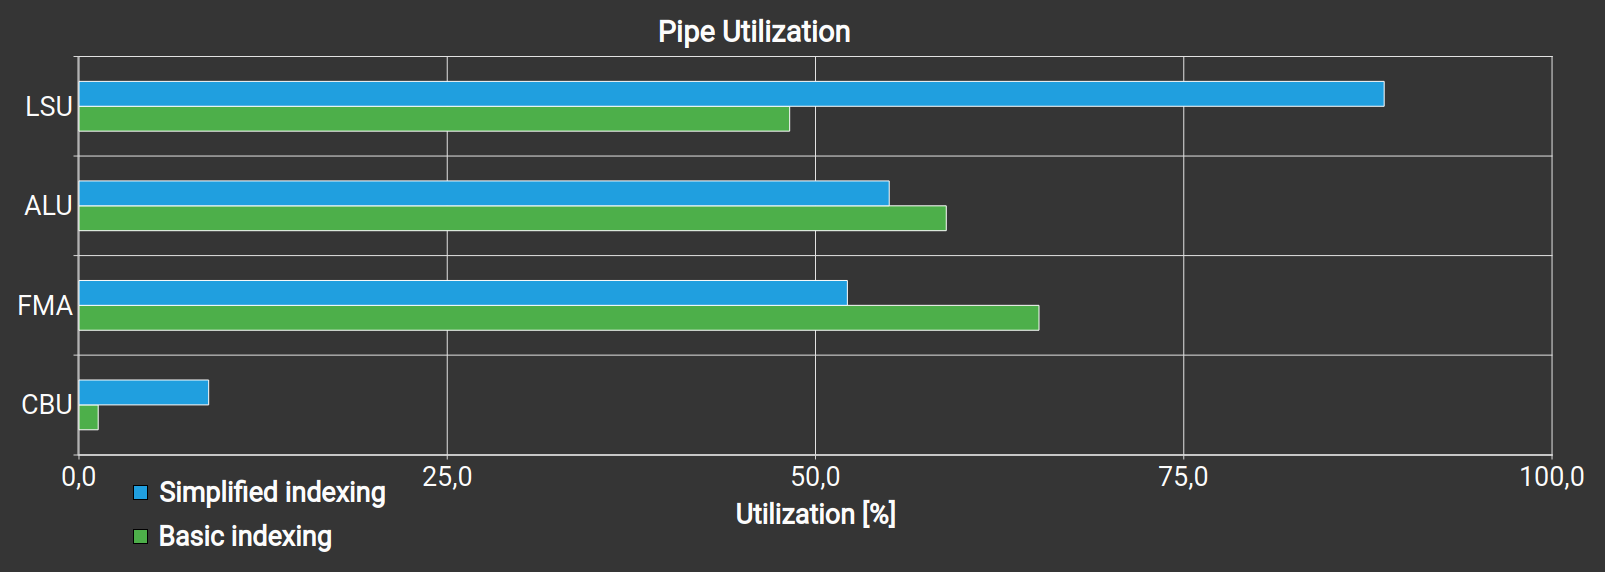
\includegraphics[width=\textwidth]{pipeline_utilization_simplified_indexing.png}
		\caption{Pipeline utilization.}
		\label{fig:pipeline_utilization_simplified_indexing}
	\end{subfigure}
	
	%\label{fig:warp_per_shift_indexing_comparison}
	\caption{Comparison of basic and simplified indexing.}
\end{figure}

The effects of different pipeline utilization can also be seen in Figure \ref{fig:warp_state_simplified_indexing}. Warps of basic indexing algorithm are mostly stalled due to not being selected, i.e. there are multiple eligible warps and only one of them can be issued. This indicates that there may be too many warps for the size of the GPU. As these benchmarks were run on a RTX 2060 mobile, which is a rather small GPU, this was to be expected. The other main reason of warp stall is \texttt{Stall Math Pipe Throttle}, which is caused by the high utilization of \textit{ALU} and \textit{FMA} pipelines. These pipelines are responsible for computing the indices and the actual results of cross-correlation, which represents the useful work done by the GPU.

Simple indexing warps on the other hand are more often stalled on the \texttt{Stall Wait}, which represents warps waiting for a fixed latency execution dependency, i.e. a data dependency between two instructions or an instruction dependency on predicate computation. We can also see noticeable increase in stalls due to access to global memory (\texttt{Stall Long Scoreboard} and \texttt{Stall LG Throttle}) together with stalls due to branching. This is consistent with the properties of simple indexing described above.

\begin{figure}[ht]
	\centering
	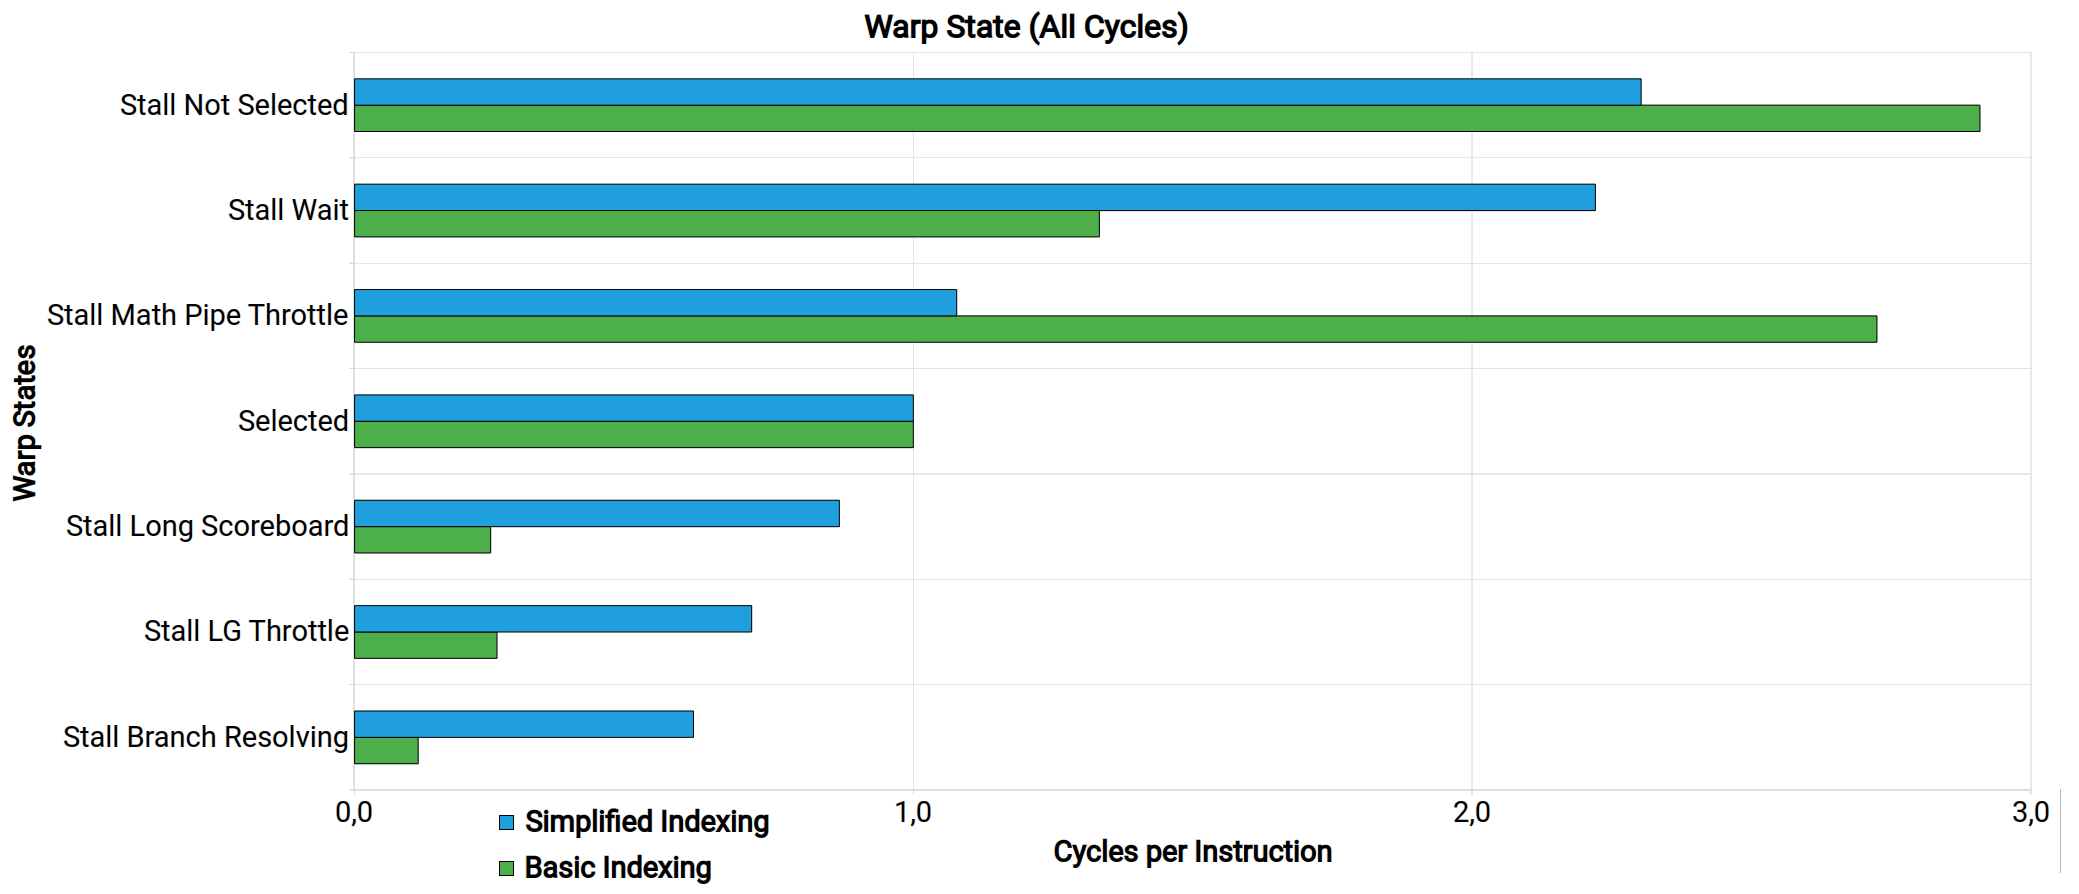
\includegraphics[width=0.8\textwidth]{warp_state_simplified_indexing.png}
	\caption{Comparison of warp stall reasons between the basic and simplified indexing.}
	\label{fig:warp_state_simplified_indexing}
\end{figure}

\subsection{Shared memory}
\label{sec:warp_per_shift_shared_mem}

This optimization takes inspiration from the warp shuffle algorithm and its \textit{multirow} optimization. Instead of sharing input values by shuffling and broadcasting across threads of a warp, we load input values into shared memory and reuse them by all warps of the thread block.

Similarly to the warp shuffle algorithm, we utilize two alternating parts forming a ring buffer for data from the left input matrix and a single buffer for data from the right input matrix. Compared to the warp shuffle algorithm,
these buffers are placed in the shared memory and are shared by all warps of each thread block. The windows of the input data loaded into buffers are not moved along the rows of the input matrices, but along a group of columns from top to bottom, processing the whole columns group before moving onto the next column group, as shown in Figure \ref{fig:shared_mem_buffer_iterations}. With appropriately sized column groups, this enables us to maximize the throughput when loading data from global memory using coalesced loads. The appropriate size here is multiple of 32, i.e. warp size.  We call this the \textit{shared\_mem\_row\_size}, as it is also the size of each row of the shared memory buffers. The number of rows in each of the three shared memory buffers (two for data from the left matrix and one for data from the right matrix) is a run-time algorithm argument and stored in variable \textit{shared\_mem\_num\_rows}.
Another reason we choose column groups instead of row groups is because of the way we assign overlaps to warps of a thread block. To prevent bank conflicts when accessing shared memory, we assign consecutive overlaps from a single column of the output matrix to the warps of a single thread block. This is explained in more detail further in this section.

\begin{figure}[ht]
	\centering
	\def\svgwidth{0.7\textwidth}
	\fontsize{8}{10}\selectfont
	% Must be relative to current directory
	% as input ignores graphicspath, which is
	% only for includegraphics{}
	\input{./img/warp_per_shift-ThreadBlockOverlapCorrect.pdf_tex}
	\caption{Computation of a single column group showcasing different warp offsets and left bottom buffer preload offset.}
	\label{fig:shared_mem_buffer_iterations}
\end{figure}



As warp shuffle algorithm had warp submatrix, i.e. submatrix of each of the input matrices containing elements required by any of the threads of the given warp, this algorithm computes thread block submatrix containing elements of the input matrices required by overlaps assigned to any of the warps of the given thread block . This thread block submatrix is what we partition into column groups and what we iterate over and load into the shared memory buffers.

The implementation is again made up of three nested for loops. The outer loop iterates over column groups, the middle loop iterates over rows of the column group in \textit{shared\_mem\_num\_rows} sized steps. Threads of the whole thread block go through these two loops synchronously to allow cooperation when loading data to the shared memory buffers. 

\begin{lstlisting}[
style=cuda
]
T thread_sum = 0;
for (
	size_t column_group_start_x = block_matrix_start.x;
	column_group_start_x < block_matrix_end.x;
	column_group_start_x += shared_mem_row_size
) {
	// Bottom part of the left shared memory buffer
	left_bottom_s.load_submatrix(...);
	
	for (
		size_t right_buffer_start_row = block_matrix_start.y;
		right_buffer_start_row < block_matrix_end.y;
		right_buffer_start_row += shared_mem_num_rows
	) {
		left_top_s.load_submatrix(...);
		right_s.load_submatrix(...);
		
		__syncthreads();
		
		compute_from_shared_mem_buffers(left_bottom_s, right_s, ...);
		
		compute_from_shared_mem_buffers(left_top_s, right_s, ...);
		
		swap(left_bottom_s, left_top_s);
		
		__syncthreads();
	}
}
\end{lstlisting}


In each iteration, we compute the parts of the right buffer which are part of the overlap assigned to the current warp and have the corresponding overlapping row from the left matrix in the given part of the left buffer, first the bottom part, then the top part.  % TODO: More detailed description

\begin{lstlisting}[
style=cuda
]
template<typename T>
__device__ void compute_from_shared_mem_buffers(
	const shared_mem_buffer<T>& left_buffer,
	const shared_mem_buffer<T>& right_buffer,
	T &thread_sum,
	...
) {
	// Offset in shared memory buffer
	int warp_right_start_offset = ...;
	int warp_right_end_offset = ...;
	
	// Offset between buffers
	int buffer_offset = ...;
	for (
		int right_idx = warp_right_start_offset + warp.thread_rank();
		right_idx < warp_right_end_offset;
		right_idx += warp.size()
	) {
		l = left_buffer[right_idx + buffer_offset];
		r = right_buffer[right_idx];
		thread_sum += l * r; 
	}
}
\end{lstlisting}

% Warps of a block compute consecutive shifts in Y axis

This innermost loop iterates over the rows from the two shared memory buffers which are overlapped in the overlap assigned to the current warp. Shared memory accesses in this loop are without bank conflicts thanks to way we assign overlaps between warps of a thread block. If we were to assign overlaps from a single row of the output matrix to warps of a thread block, as is done by the basic implementation of \textit{warp per shift} algorithm, we would encounter a problem illustrated in Figure \ref{fig:warp_per_shift_shared_mem_overlaps_in_x}. For the purposes of this example, we work with warps of 4 threads, shared memory with 4 banks and assume each input matrix fits into one shared memory buffer. The figure shows the left and right input matrix and how their elements map into banks of shared memory when loaded by the thread block. For simplicity, we have chosen a thread block whose thread block submatrix contains whole input matrices as one of the overlaps computed by the thread block is the overlap with shift $[0, 0]$. When warps of a given thread block are assigned overlaps along a row of the output matrix, the overlaps differ in the number of columns. This leads to an access pattern with different stride in each warp. The strides for warps 1 and 2 result in 2-way bank conflicts, the stride for warp 0 results in 4-way bank conflict. With 32 threads per warp, this type of access would cause up to 32-way bank conflict, which would severely limit the shared memory throughput.


\begin{figure}[ht]
	\centering
	\def\svgwidth{0.4\textwidth}
	\fontsize{8}{10}\selectfont
	% Must be relative to current directory
	% as input ignores graphicspath, which is
	% only for includegraphics{}
	\input{./img/warp_per_shift-SharedMemAlongX.pdf_tex}
	\caption{Input matrices with numbers designating their mapping to shared memory banks and how they are accessed by 4 different warps of a single thread block in iteration 1 when assigned along a row of the output matrix.}
	\label{fig:warp_per_shift_shared_mem_overlaps_in_x}
\end{figure}

Due to this, we choose to assign overlaps from a single column to warps of a thread block. This assignment leads to access illustrated in Figure \ref{fig:warp_per_shift_shared_mem_shifts}. This figure depicts two iterations of the innermost loop, with the same simplifications as the previous figure.  As the overlaps differ in the number of rows, not columns, the access to shared memory has different starting and ending offset, but between these the access is perfectly linear and coalesced, each thread accessing different bank. Left buffer is accessed independently of the right buffer, so sharing banks between these buffers does not lead to bank conflicts.


\begin{figure}[ht]
	\centering
	\def\svgwidth{0.7\textwidth}
	\fontsize{8}{10}\selectfont
	% Must be relative to current directory
	% as input ignores graphicspath, which is
	% only for includegraphics{}
	\input{./img/warp_per_shift-SharedMemAlongY.pdf_tex}
	\caption{Input matrices with numbers designating their mapping to shared memory banks and how they are accessed by 4 different warps of a single thread block in the first two iterations when assigned along a column of the output matrix.}
	\label{fig:warp_per_shift_shared_mem_shifts}
\end{figure}

When loading the bottom part of the left shared memory buffer directly in the outer loop, we need to limit which rows are loaded to the buffer and offset the loaded rows, as shown in Figure \ref{fig:shared_mem_buffer_iterations}. If we were to just load the full buffer as shown in Figure \ref{fig:left_buffer_no_preload}, we would encounter a situation where rows loaded in the second iteration of the middle loop into the right buffer overlap rows which were loaded during the first load of bottom left buffer, which at that point is already overwritten.  


\begin{figure}[ht]
	\centering
	\def\svgwidth{0.4\textwidth}
	\fontsize{8}{10}\selectfont
	% Must be relative to current directory
	% as input ignores graphicspath, which is
	% only for includegraphics{}
	\input{./img/warp_per_shift-ThreadBlockOverlapsWrong.pdf_tex}
	\caption{Cross-iteration dependency when the load of the bottom part of the left buffer is not limited and offset.}
	\label{fig:left_buffer_no_preload}
\end{figure}

% 	Its basically very similar to multirow optimization, just with workers of warp size
% 	And because they are warp size, we can compute bounds for each and stop them whenever
%	we need without thread divergence
Even with the throughput of shared memory, the load from shared memory \textit{LDS} instructions become a bottleneck, as shown in Figure \ref{fig:warp_state_shared_mem}. The memory input/output stall is caused by the memory input/output queue being full. This queue handles special math instructions, dynamic branches and most importantly for us the shared memory access instructions.

\begin{figure}[ht]
	\centering
	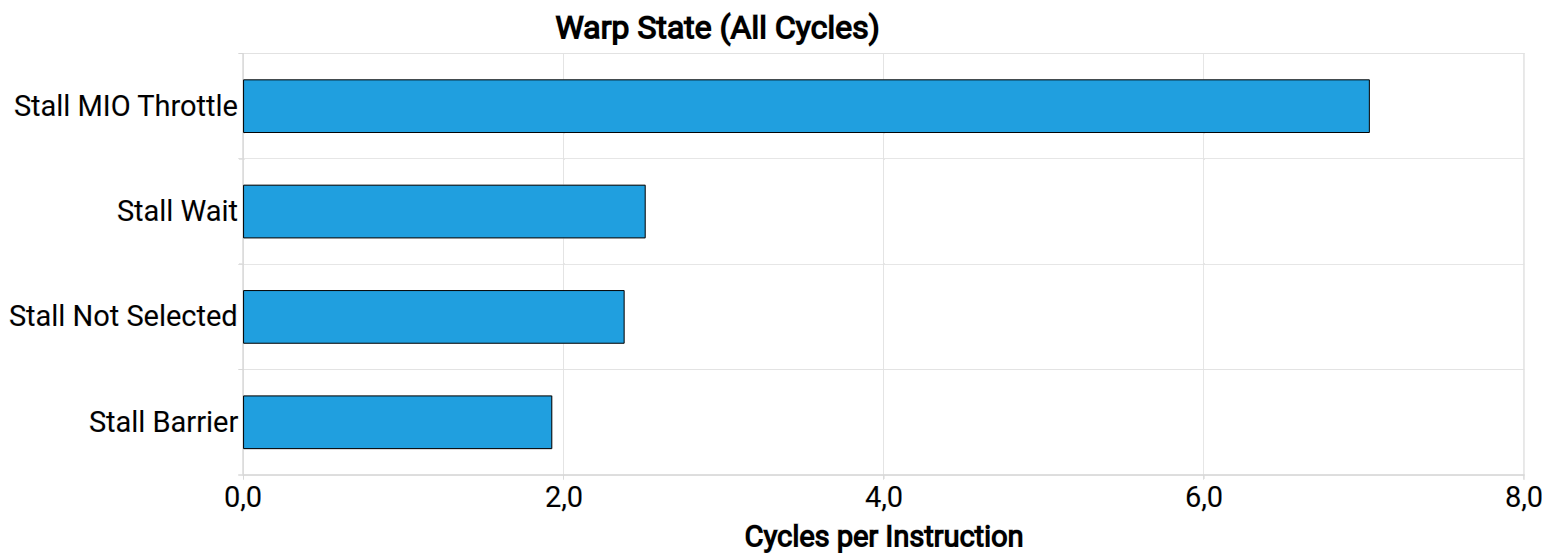
\includegraphics[width=0.8\textwidth]{warp_state_shared_mem.png}
	\caption{Memory input/output (MIO) stall caused by excessive shared memory access.}
	\label{fig:warp_state_shared_mem}
\end{figure}

\subsection{Loading data to shared memory}

When loading data to shared memory, we have a choice between two different access patterns, shown in Figure \ref{fig:shared_memory_loading_patterns}:
\begin{itemize}
	\item strided warps,
	\item continuous warps.
\end{itemize}

\begin{figure}[ht]
	\centering
	\def\svgwidth{0.4\textwidth}
	\fontsize{8}{10}\selectfont
	% Must be relative to current directory
	% as input ignores graphicspath, which is
	% only for includegraphics{}
	\input{./img/warp_per_shift-SharedMemLoading.pdf_tex}
	\caption{Difference between strided and continuous loading patterns.}
	\label{fig:shared_memory_loading_patterns}
\end{figure}

With strided warps, each warp loads chunks of \textit{warp size} items with stride of \textit{thread block size} items. 
%\[ \left[i * block\_size + w * warp\_size, i * block\_size + (w + 1) * warp\_size\right) \]

With continuous warps, the whole block of data is divided into equal parts, one for each warp. Each warp then loads the single continuous part of the data. The advantage compared to strided loads is that this access pattern should better utilize caches, as each warp does sequential access. The disadvantage is mainly in the fact that each warp will load some part of the data, even if the data is small and could be loaded by a subset of warps with strided loading. % TODO: Benchmark results

\subsection{Shared memory with multiple right matrices}

Similarly to the warp shuffle algorithm, we can increase the ratio of arithmetic instructions to shared memory loads by computing the same shift between a single left matrix and multiple right matrices. This optimization is limited by the size of shared memory, as we need to fit multiple right shared memory buffers described in the previous section into shared memory at once. The code changes are very similar to the warp shuffle changes. We change the \textit{thread\_sum} and \textit{right\_s} variables into arrays and wrap every access into an unrollable for loop. As we are again computing overlaps with the same shift from different output matrices, any loop bounds computed hold for all the overlaps.

% TODO: Maybe code

The effects of this optimization are shown in Figure \ref{fig:shared_memory_multimat_right_profiling}. The number of shared memory load instructions (LDS) and memory access index computations using the integer multiply-add (IMAD) is significantly reduced. Even with this reduction, the utilization of the \textit{LSU} pipeline is still a bottleneck, most likely due to the reduced throughput of shared memory in the Compute Capability 7.5 we use for profiling. The higher utilization of \textit{FMA} pipeline hints at better performance, which will be shown in Section \ref{sec:results_shared_mem}.


\begin{figure}[ht]
	\centering	
	\begin{subfigure}{0.8\textwidth}
		\centering
		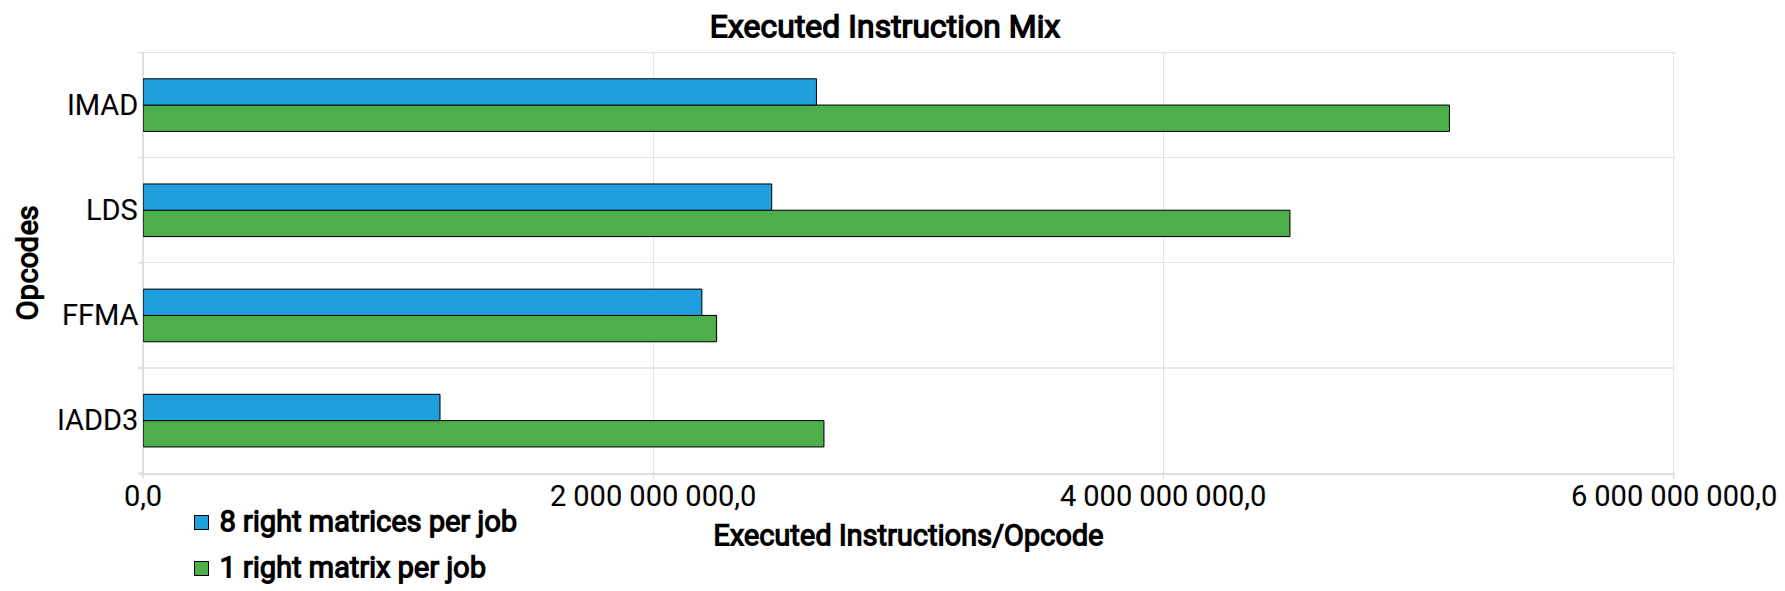
\includegraphics[width=\textwidth]{executed_instructions_shared_mem.png}
		\caption{Executed instructions.}
		%\label{fig:executed_instructions_shared_mem}
	\end{subfigure}
	\hfill
	\begin{subfigure}{0.8\textwidth}
		\centering
		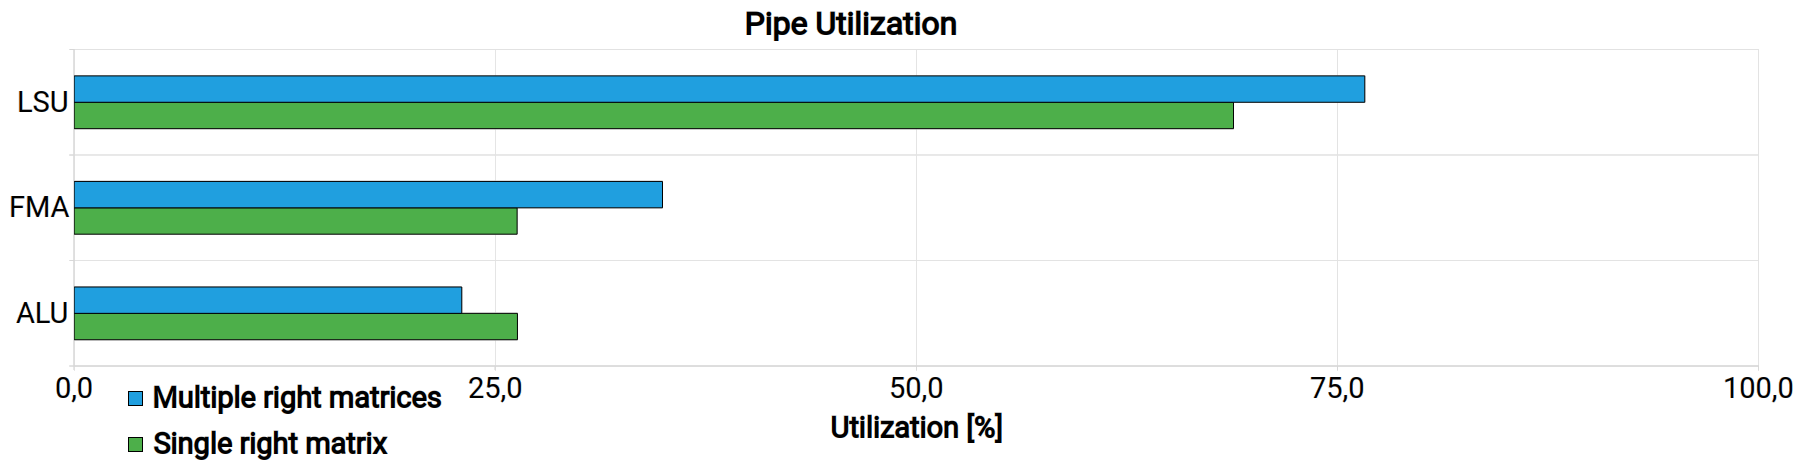
\includegraphics[width=\textwidth]{pipeline_utilization_shared_mem.png}
		\caption{Pipeline utilization.}
		%\label{fig:pipeline_utilization_shared_mem}
	\end{subfigure}
	
	\caption{Profiling of the effects of multiple right matrices on shared memory optimization.}
	\label{fig:shared_memory_multimat_right_profiling}
\end{figure}

\subsection{Shared memory with single column group per block}
\label{sec:column_group_per_worker}
As described in Section \ref{sec:warp_per_shift_shared_mem}, the thread block matrix is split into column groups. Each of these column groups can be processed independently, with the partial result added to the total using \textit{atomicAdd} instruction as is done for work distribution in warp shuffle algorithm, described in Section \ref{sec:warp_shuffle_work_dist}. This optimization borrows from the rectangle work distribution, first computing the maximum number of column groups per shifts $m$ and then starting $m$ workers for each shift.

We utilize the \textit{z} dimension of the grid size to multiply the number of workers by $m$. Based on thread block \textit{z} index, each warp computes its assigned column group of the given thread block matrix. The loop bounds are computed to only include the assigned column group, after which the code from the original implementation with multiple column groups can be reused without any changes.

\subsection{Work distribution}

As described in Section \ref{sec:warp_shuffle_work_dist} with the warp shuffle algorithm, there are massive differences between work done by different workers in the basic algorithm. The implementation shares much of the code with the warp shuffle algorithm, only difference being the size of workers. We can choose from the \texttt{triangle} or \texttt{rectangle} distributions and set the maximum number of rows processed by a worker.

In our benchmarks using RTX 2060 GPU, this optimization was only beneficial for inputs smaller than 32 by 32, as shown in Figure \ref{fig:warp_per_shift_work_dist_local_results}. For larger inputs, the GPU is already saturated and with each warp processing a single shift, the workload per thread is already small enough that the work distribution does not bring any noticeable improvement. Additionally, without the use of shared memory described in Section \ref{sec:warp_per_shift_shared_mem}, the added load onto global memory makes this implementation slower for larger inputs.

With larger GPUs, the boundary where the benefits of increased occupancy are diminished by added strain onto global memory is moved onto larger inputs, as is shown in Figure \ref{fig:warp_per_shift_work_dist_gpulab}. % TODO: Benchmark on GPU lab


% TODO: Maybe switch to kernel runtime from total computation time
\begin{figure}[ht]
	\centering
	\def\svgwidth{0.4\textwidth}
	% Must be relative to current directory
	% as input ignores graphicspath, which is
	% only for includegraphics{}
	\input{./img/warp_per_shift_work_dist_local_results.pdf_tex}
	\caption{Comparison of computation time between simplified warp per shift algorithm, warp per shift with shared memory and warp per shift with work distribution.}
	\label{fig:warp_per_shift_work_dist_local_results}
\end{figure}



\subsection{Block per shift}

Another possible way to further increase occupancy is to switch from warps as workers to whole thread blocks as workers. This can massively increase the number of threads started for given size of input, saturating the GPU even for smaller inputs.
The implementation is rather simple. The thread block index directly maps to the position in the output matrix and consequently to the overlap computed by given thread block. We then compute the bounds of the overlapping submatrix and iterate over the overlapping elements using block stride loop. We then utilize \texttt{reduce} function provided by Cooperative Groups API to sum results in each warp, which are then stored into shared memory and reduced again by warp 0. The final result is then stored into the output matrix.

Based on our testing with RTX 2060, the block per shift algorithm does not significantly improve the run time over the simple warp per shift algorithm even for small input matrices, as shown in Figure \ref{fig:block_per_shift_local_results}. This is most likely caused by the simple warp per shift algorithm already saturating the GPU. 

\begin{figure}[ht]
	\centering
	\def\svgwidth{0.4\textwidth}
	% Must be relative to current directory
	% as input ignores graphicspath, which is
	% only for includegraphics{}
	\input{./img/block_per_shift_local_results.pdf_tex}
	\caption{Comparison of the simple warp per shift algorithm and block per shift algorithm.}
	\label{fig:block_per_shift_local_results}
\end{figure}

For larger GPUs, this implementation may be beneficial, but may also suffer from the low workload per thread, unbalanced workload between workers and no data reuse.

% TODO: Benchmark on GPULab


